% 论文入口。沿用原 cumcmthesis.cls / cumcm2026.sty；原 example.tex 未覆盖。
% 建议用户在本目录用 XeLaTeX 编译两次。本次仅提供源稿，不编译。
\documentclass[withoutpreface,bwprint]{cumcmthesis}
\usepackage{cumcm2026}
\usepackage{url}
\usepackage{placeins}
\hypersetup{hidelinks}
\setlength{\emergencystretch}{2em}
\renewcommand{\arraystretch}{1.13}
\title{非对称结算机制下的微网采购与储能协同调度}
\tihao{C}
\yearinput{2026}
\monthinput{9}
\dayinput{10}

\begin{document}
\maketitle
\begin{abstract}
针对微网采购、储能与预测更新的协同问题，建立以实际结算费用为中心的统一调度框架。由五倍紧急补购及1.5倍上调收费，推导无储能单时段的80\%日前采购分位数、70\%条件上调阈值及动态价格下的加权分位数，解释采购偏高的经济动机，再将该机制嵌入含功率、容量和效率限制的场景优化。

问题一建立购电与储能联合线性规划，并利用免费弃余条件证明存在不同时充放电的最优解。计算得到全天计划购电59482.70 kWh、购电费35126.95元，较无储能基准节省26.90\%，首末储电量均为6000 kWh。

问题二以一月实际账单校准有限候选预测器和执行器，冻结后对2月至12月334天顺序回测。主案保留此前28日完整残差轨迹，关闭额外风险与备用。总费用1401.28万元，较相同预测及初态下的点预测方案节省8.36\%，紧急购电85017.69 kWh。固定与自适应风险、备用单独及联合对照显示，附加保守机制并不普遍节费。

问题三将0、6、12、18时的合同修订与每10分钟的储能控制分开，另实现固定合同的内层LP及跨日续接候选。其一月费用未优于规则执行，故主案仍使用经校准的规则，总费用1397.58万元，紧急购电12647.76 kWh。通过同计划场景回放量化规划与执行偏差，并以SOC、新光伏和负荷反馈的递进对照识别更新收益，避免将参考调度等同于真实控制。

问题四以同日价荷残差构造联合场景，按真实价格结算，静态与滚动策略费用分别为1479.41万元和1476.92万元，紧急电量分别为80544.00和11950.68 kWh。本文区分实际账单、规划回放偏差与可选风险偏好，明确退款、终端库存及未来修订机会的近似边界。所有表格与附件5由统一物理时间索引和同一执行结果生成，保留完整源代码及原模板。

\keywords{微网调度\quad 非对称结算\quad 采购分位数\quad 场景优化\quad 因果储能控制}
\end{abstract}

\section{问题重述与分析}

微网利用储能转移电量，并根据外网收费规则决定提前采购及补购。本题的目标是在满足负载、容量及功率限制的条件下尽可能节省实际购电费用。问题一给定单日输入，建立确定性日前联合线性规划作为物理基础\cite{kong2016,silva2020}。问题二引入负载与光伏的不确定性，五倍紧急电价和无退款的计划费用构成非对称预测误差成本，采用历史残差场景进行采购\cite{abunima2022,marino2018,grover2018}。问题三在规定发布时点允许付费修订，进一步区分常规购电承诺与10分钟储能控制\cite{palma2013,silvente2015,li2016,jani2022}。问题四保留上述结构，通过联合残差刻画价格与净负荷的关联\cite{li2020}。

四问的主路线为“确定性LP、非对称结算下的场景采购、交易约束下的双时间尺度控制、价荷联合不确定下的滚动调度”。本文用收费机制解释采购行为，并核对优化参考计划和实际控制所产生的费用。CVaR、备用及内层LP均接受实际账单检验。风险项与备用在经济主方案中关闭；一月校准四案均选中因果贪心执行器，因此内层LP作为已实现的候选及对照，不能写成必然优于原控制规则的主结论。

\section{模型假设与符号说明}

\subsection{基本假设}

\begin{enumerate}
 \item 将源文件功率解释为以标记时刻为右端点的10分钟平均功率，以$\Delta t=1/6$小时换算电量。这是时间离散的建模解释，不是赛题明确给出的事实。忽略线路损耗及自放电，充电、放电效率分别为$\eta_c=\eta_d=0.9$，往返效率为0.81。
 \item 不售电，富余电量允许免费弃置。主口径下计划购电全额付费，取消部分不退款；退款解释仅用于敏感性分析。不引入题目未给出的折旧、碳成本或投资费用。
 \item 储电量保持在1200--10800 kWh，充放电功率均不超过5000 kW。问题一首末储电量均为6000 kWh；其他问题仅在1月1日初始化，以后连续传递状态。
 \item 每10分钟可观测当期负载、光伏、电价及储电量并完成平衡。紧急购电可补足剩余缺口，不另设题目未给出的容量上限。未来实际值不可提前使用，附件4全天实际价格不作为日前已知输入。
\end{enumerate}

\subsection{主要符号}

购电量和电池外侧充放电量统一使用kWh，以$p$表示电价、$c$表示充电量。
\begin{table}[htbp]
\centering\small
\caption{主要符号及含义}\label{tab:symbols}
\begin{tabularx}{\linewidth}{p{0.18\linewidth}Xl}
\toprule
符号 & 含义 & 单位\\
\midrule
$D,t,s$ & 日期、日内时段$t=0,\ldots,143$、场景索引 & ---\\
$L_{D,t},R_{D,t},n_{D,t}$ & 实际负载功率、光伏功率、净负荷电量 & kW、kW、kWh\\
$p_{D,t}$ & 实际交易电价 & 元/kWh\\
$g_{D,t},a_{D,t}$ & 零时原计划、最终有效常规购电量 & kWh\\
$c_t,d_t,e_t$ & 电池外侧充电量、放电量、时段初储电量 & kWh\\
$h_t,w_t$ & 紧急购电量、弃置电量 & kWh\\
$\pi_s,Q_s$ & 场景概率、场景剩余时域紧急费用 & ---、元\\
$\rho_t,\lambda$ & 外层参考备用量、CVaR权重 & kWh、---\\
$\beta_T,k_\rho$ & 终端偏离惩罚系数、备用缩放系数 & 元/kWh、---\\
$E_{\min},E_{\max},U$ & 储电量下上限、单段电量上限$5000/6$ & kWh\\
\bottomrule
\end{tabularx}
\end{table}

\section{数据处理与因果预测}

\subsection{统一物理时间索引与原模板映射}

每天保留144段，定义
\begin{equation}
 I_t=[t/6,(t+1)/6),\qquad n_{D,t}=(L_{D,t}-R_{D,t})/6.
 \label{eq:time_energy}
\end{equation}
源标记00:10对应物理00:00--00:10，$0{:}00{+}1$对应物理23:50--24:00，最后一段归入当天结算。附件5按要求保留原有表头，从0:10--0:20开始，以次日0:00--0:10结束；按源样本列序写入，不因表头再平移数据。

映射冻结于\texttt{data/time\_mapping.json}：每个$t$同时记录源时间、物理区间、模板标签、单元格位置及四小时分组。指定时段表、储能汇总、紧急区间和工作簿均从同一索引生成。例如$t=60$对应源10:10、物理10:00--10:10、模板10:10--10:20；题目指定的10:00--10:10结果取$t=60$，而不按模板文字反查。紧急区间按物理连续时段合并，四小时汇总按连续24段求和。这一区分使论文自然日结算与原模板显示均可追溯。

\subsection{一月费用校准与固定运行前缀}

修订模型以1月15--31日为验证窗口，按实际结算费用选择预测器及控制器，2月1日--12月31日334天用于评价与填报。所有同一问题的验证候选从已冻结旧版策略在1月15日的实际储电量出发，各自连续运行至1月31日。候选的期末电量同时报告，但不作为虚拟退款冲减验证费用，因此这是账单比较，并非库存价值已经中和的比较。

候选集合预先限定：问题二、三的负载在前一周、最近2个及4个同星期日均值间选择；问题二的历史光伏在3、7、14日均值间选择。动态电价两案继承对应固定价问题选定的负载及光伏预测器，再在上述三类同星期方法中选择价格预测器。采用逐项坐标搜索，先固定28场景、无风险和无备用的内层LP配置选择预测，再比较贪心与内层LP控制器；滚动两案另比较启用跨日续接的LP。该有限候选搜索不等同于预测与控制全部组合的全局最优。风险及备用关闭、终端系数倍率1等未搜索设置明确固定。四案控制器均由一月账单选中贪心规则，结果及库存边界见下表。

\begin{table}[htbp]\centering\small
\caption{一月验证冻结的预测配置与执行结果}
\label{tab:v2_forecast_selection}
\begin{tabularx}{\linewidth}{LLLLRR}\toprule
问题 & 负荷 & 光伏 & 电价 & 验证费/元 & 末库存/kWh\\\midrule
问题2 & 同星期2日 & 最近3日 & 已知电价 & 917318.59 & 7155.31\\
问题3 & 同星期2日 & 附件3发布值 & 已知电价 & 919340.82 & 7143.30\\
问题4-2 & 同星期2日 & 最近3日 & 同星期4日 & 1042234.20 & 7298.41\\
问题4-3 & 同星期2日 & 附件3发布值 & 同星期2日 & 1043044.13 & 7308.72\\
\bottomrule\end{tabularx}
\par\smallskip\parbox{\linewidth}{\footnotesize 验证期为1月15日至31日；所有主案选择规则执行、28个历史场景，额外CVaR与备用均关闭。预测器先以统一储能LP进行逐坐标费用比较，再比较执行器，属于有限候选搜索。}
\end{table}

正式2月初态承接各问题已经冻结的旧版1月运行末态，同一问题所有修订策略使用相同初态；不会用1月底才选定的方法回写1月运行以改变2月库存。随后实际末态逐日传递。旧版1月记录仅作为共同运行前缀，1月验证模拟用于选型，两者用途不同。尽管2--12月数据不进入此次选型目标，修订研究已参考过旧版该时段结果，因此本文称其为冻结规则后的顺序回测，不称为从未接触的独立测试。

\subsection{预测更新及误差评价}

令$X$表示负载或价格，同星期预测使用已完成的历史日：
\begin{equation}
 \widehat X_{D,t}=\frac{1}{|\mathcal W_D|}\sum_{j\in\mathcal W_D}X_{j,t},\quad
 \mathcal W_D=\{D-7i:i=1,\ldots,K\}\cap\{1,\ldots,D-1\}.
 \label{eq:weekday_forecast}
\end{equation}
移动均值则取此前$K$个完整日。历史不足使用已有样本，无相应星期日时退回近7日均值，首日固定使用附件1先验。历史预测的每个日期均只读取此前数据；全年数组的预先生成不改变这一信息限制。

滚动问题使用当次已发布的24点光伏预报，将发布时刻$r$后第1至24个小时作为预报横坐标，以发布时刻已知光伏值为锚点线性插值到10分钟右端点。日内负载与动态电价用此前2小时的平均预测偏差$b_r$修正：
\begin{equation}
 \widehat X_{r,k}=\max\{\ell_X,\widehat X^{(0)}_{r,k}
 +\operatorname{clip}(b_r e^{-k/36},-0.3\widehat X^{(0)}_{r,k},0.3\widehat X^{(0)}_{r,k})\}.
 \label{eq:issue_correction}
\end{equation}
其中$k$为发布后的步数，负载下界$\ell_X=0$，预测价格下界为$10^{-6}$元/kWh。6小时衰减尺度和30\%幅度事先固定。只在0、6、12、18时更新这组预测，其他时刻的内层LP候选仅替换当前一步实际值，不使用尚未发布的光伏预报。

预测误差报告$\mathrm{RMSE}=\sqrt{N^{-1}\sum_i(X_i-\widehat X_i)^2}$及$\mathrm{MAE}=N^{-1}\sum_i|X_i-\widehat X_i|$。表中2--12月指标只作描述，不重新选型；滚动问题另外报告零时发布光伏预报的误差，避免与未用于其采购的历史光伏预测混淆。
\begin{table}[htbp]\centering\small
\caption{已选预测器的误差指标（光伏发布值取零时版本）}
\label{tab:v2_forecast_metrics}
\begin{tabularx}{\linewidth}{LLRRRR}\toprule
问题 & 变量 & 一月MAE & 一月RMSE & 评价期MAE & 评价期RMSE\\\midrule
问题2 & 负荷/kW & 122.51 & 152.09 & 171.91 & 240.54\\
问题2 & 光伏/kW & 100.38 & 214.94 & 154.46 & 313.48\\
问题3 & 负荷/kW & 122.51 & 152.09 & 171.91 & 240.54\\
问题3 & 光伏/kW & 135.37 & 266.89 & 197.49 & 383.03\\
问题4-2 & 负荷/kW & 122.51 & 152.09 & 171.91 & 240.54\\
问题4-2 & 光伏/kW & 100.38 & 214.94 & 154.46 & 313.48\\
问题4-2 & 电价/(元/kWh) & 0.03390 & 0.04364 & 0.04886 & 0.06963\\
问题4-3 & 负荷/kW & 122.51 & 152.09 & 171.91 & 240.54\\
问题4-3 & 光伏/kW & 135.37 & 266.89 & 197.49 & 383.03\\
问题4-3 & 电价/(元/kWh) & 0.03434 & 0.04386 & 0.04515 & 0.06383\\
\bottomrule\end{tabularx}
\par\smallskip\parbox{\linewidth}{\footnotesize 一月指1月15日至31日；评价期指2月至12月。评价期误差仅作结果描述，不参与选型；价格列与功率列单位不同。}
\end{table}

\section{结算机制与采购行为}
\label{sec:settlement_mechanism}

\subsection{先固定结算口径，再比较策略}

赛题规定计划购电按计划量计费，上调部分按交易电价的1.5倍支付，下调部分按交易电价的50\%承担违约费用，紧急购电按5倍电价支付。对取消的原计划是否返还原购电费，文字没有另行给出退款项。本文主方案采用原计划全额付费且不退款的解释，同时将退款解释作为敏感性对照。两种解释下的单时段非紧急费用见表\ref{tab:mech_settlement_convention}，其中$[x]_+=\max\{x,0\}$，$g$为零时原计划，$a$为最终有效常规购电量。

\begin{table}[htbp]
\centering
\caption{结算口径对比与单时段示例（不含紧急购电费）}
\label{tab:mech_settlement_convention}
\small
\begin{tabularx}{\linewidth}{p{0.18\linewidth}Xrr}
\toprule
口径 & 非紧急费用 & 下调示例 & 上调示例\\
\midrule
主口径：不退款 & $pg+1.5p[a-g]_++0.5p[g-a]_+$ & 110元 & 130元\\
退款敏感性口径 & $p\min\{g,a\}+1.5p[a-g]_++0.5p[g-a]_+$ & 90元 & 130元\\
\bottomrule
\end{tabularx}
\par\smallskip
\begin{minipage}{\linewidth}
\footnotesize 注：两例均取$g=100$ kWh、$p=1$元/kWh；下调例取$a=80$ kWh，上调例取$a=120$ kWh。退款解释仅在下调时返还取消部分的原计划费用。
\end{minipage}
\end{table}

在任一口径下，紧急费用均另加$5ph$，多次修订均与零时原计划比较，并按最后生效的购电量结算，不对相邻修订重复收费。历史负载、光伏和价格数据只能用于评估给定结算定义下的策略结果，不能凭数值结果反证结算定义，更不能因退款解释费用较低就选择该口径。后文的主结果与退款敏感性结果分别汇报。

相同修订策略在两种口径下的334天费用相差320347.51元，其量级大于若干控制增强的收益。因此先固定结算语义，再解释模型改进；完整敏感性结果见表\ref{tab:v2_settlement}。

\paragraph{不退款口径下的下调支配性。}
假设$p>0$、原计划不退款且富余电量允许免费弃置。若某可行解有$a<g$，把有效购电量改为$a'=g$，保持原充放电、紧急购电及储电轨迹不变，将新增的$g-a$电量弃置，物理约束仍满足，结算费用减少$0.5p(g-a)>0$。因此至少存在一个满足$a\ge g$的最优解。该结论依赖上述三个条件，在表\ref{tab:mech_settlement_convention}的退款解释下不能直接使用。对固定购电量的内层储能控制器而言，此结论也不授权其修改外层已经承诺的购电量。

\subsection{五倍补购价格导出的80\%采购分位数}

为解释采购的经济动机，先剥离储能及跨时段约束。设$X$为单时段实际净需求电量，可以为负；$q\ge0$为提前承诺的采购量，$p>0$为确定电价，富余电量无残值，且$\mathbb E[X_+]<\infty$。给定决策时已有的信息，以下概率和期望均针对当时可得的条件分布。期望结算费用为
\begin{equation}
 J_2(q)=pq+5p\,\mathbb E[(X-q)_+].
 \label{eq:mech_q2_cost}
\end{equation}
记$F_X(x)=\Pr(X\le x)$、$F_X(x^-)=\Pr(X<x)$。函数$J_2$为凸函数，其次梯度区间为
\begin{equation}
 \partial J_2(q)=p[5F_X(q^-)-4,\ 5F_X(q)-4].
 \label{eq:mech_q2_subgradient}
\end{equation}
对于$q>0$的内点最优解，充要条件是
\begin{equation}
 F_X(q^-)\le0.8\le F_X(q).
 \label{eq:mech_q2_quantile_condition}
\end{equation}
这同时适用于连续分布和含原子的离散场景分布。若分布在最优点连续，则有$J_2'(q)=p-5p\Pr(X>q)=0$，即$F_X(q)=0.8$；若最优点位于$q=0$边界，则右导数非负的条件为$F_X(0)\ge0.8$。定义下分位数$F_X^{-1}(\alpha)=\inf\{x:F_X(x)\ge\alpha\}$，可选取
\begin{equation}
 q_2^\star=\max\{0,F_X^{-1}(0.8)\}.
 \label{eq:mech_q2_quantile}
\end{equation}
若分布存在平坦区间，最优解可能不唯一，该式给出其中一个可行选择。

因此，五倍补购价格本身就使低估需求的经济损失高于高估需求的损失。即便仅最小化期望费用、完全不加入CVaR，最优采购也可能高于均值。采购偏高不能单独作为风险厌恶的证据，风险扩展是否值得保留仍应由额外费用及其带来的可观察收益判断。

\subsection{1.5倍增购价格导出的70\%条件阈值}

在主结算口径下，固定零时计划$g\ge0$，由下调支配性只需研究$a\ge g$的增购决策。将已经承诺的$pg$视为常数，当前剩余费用为
\begin{equation}
 J_3(a)=1.5p(a-g)+5p\,\mathbb E[(X-a)_+],\qquad a\ge g.
 \label{eq:mech_q3_cost}
\end{equation}
同理，$\partial J_3(a)=p[5F_X(a^-)-3.5,\ 5F_X(a)-3.5]$。当$a>g$时，最优条件为$F_X(a^-)\le0.7\le F_X(a)$；在$a=g$边界，条件为$F_X(g)\ge0.7$。因此可取
\begin{equation}
 a_3^\star=\max\{g,F_X^{-1}(0.7)\}.
 \label{eq:mech_q3_quantile}
\end{equation}
式\eqref{eq:mech_q3_quantile}中的分布必须由修订时已经获得的信息确定。70\%是给定原计划后的单时段增购阈值，不是问题三零时计划的最优分位数，也不表示增购量直接等于需求的70\%分位数。实际增购量为$[F_X^{-1}(0.7)-g]_+$。零时计划如要计入以后修订的价值，还需描述未来信息到达及合法修订决策，不能由这一单时段推导替代。

\subsection{波动价格下的价格加权需求分位数}

若未来结算电价$P$也未知，设$P>0$几乎处处成立，$0<\mathbb E[P]<\infty$，且$\mathbb E[PX_+]<\infty$。单时段日前决策在当时信息下固定$q$，期望费用为
\begin{equation}
 J_4(q)=\mathbb E[P]q+5\mathbb E[P(X-q)_+],\qquad q\ge0.
 \label{eq:mech_q4_cost}
\end{equation}
定义价格加权分布
\begin{equation}
 G(x)=\frac{\mathbb E[P\,\mathbf 1_{\{X\le x\}}]}{\mathbb E[P]},\qquad
 G(x^-)=\frac{\mathbb E[P\,\mathbf 1_{\{X<x\}}]}{\mathbb E[P]}.
 \label{eq:mech_weighted_cdf}
\end{equation}
由$P>0$和有限期望，$G$是合法分布函数，并有
\begin{equation}
 \partial J_4(q)=\mathbb E[P][5G(q^-)-4,\ 5G(q)-4].
 \label{eq:mech_q4_subgradient}
\end{equation}
内点最优条件为$G(q^-)\le0.8\le G(q)$，在连续点化为$\mathbb E[P\mathbf 1_{\{X\le q\}}]/\mathbb E[P]=0.8$。考虑非负约束，可取
\begin{equation}
 q_4^\star=\max\{0,G^{-1}(0.8)\}.
 \label{eq:mech_weighted_quantile}
\end{equation}
在离散场景$(x_s,p_s,\pi_s)$下，$p_s>0$、$\pi_s\ge0$、$\sum_s\pi_s=1$，只需把场景概率改写为
\begin{equation}
 \widetilde\pi_s=\frac{\pi_sp_s}{\sum_j\pi_jp_j},\qquad
 G(x)=\sum_{s:x_s\le x}\widetilde\pi_s.
 \label{eq:mech_scenario_reweight}
\end{equation}
若$P$与$X$独立，则$G=F_X$，退化为普通80\%分位数；若高需求经常伴随高价格，相应场景在采购决策中的权重增大。该机制说明，问题四应保留价格与净负荷的联合关系，分别打乱两类历史残差会改变优化问题所使用的经济权重。

\subsection{与储能联合优化及预测评价的衔接}

以上阈值是无储能单时段子问题的解析基准。加入储能后，当前多购或少购的影响会通过充放电效率、容量、功率及后续电价传递到其他时段，电池存量具有随时间和状态变化的机会价值。因此，80\%和70\%不能直接逐时套用于完整调度，也不能为参考备用公式中的80\%误差分位数提供理论背书。参考备用参数和采购分位数具有不同的决策对象与约束作用，应分别检验。

本文据此将模型递进关系明确为：结算规则决定非对称误差成本，场景采购刻画这种成本，再由储能联合优化处理跨时段耦合，实际控制在已经承诺的常规购电量和合法信息范围内执行。经济主方案以实际总购电费用为评价依据，CVaR和参考备用作为可选运行偏好，与期望费用策略在相同条件下比较。终端价值近似系数记为$\beta_T$，单位为元/kWh；备用缩放系数记为$k_\rho$，为无量纲数，二者不复用符号。

预测评价也应对应这一经济目标。文献\cite{elmachtoub2017spo}提出以预测引致的决策损失评价预测，并进一步构造SPO与SPO+方法。
% Citation locator: https://arxiv.org/abs/1710.08005, Abstract paragraphs 1--2.
本文仅借鉴其决策导向思想：在相同历史信息、初始储电量、场景构造和控制器下，将候选预测器输入统一调度程序，以一月逐日实际结算费用选择预测方法，RMSE和MAE作为描述性指标。在预测器选型后再比较控制器，属于有限候选集上的分步验证，不等同于实现SPO或SPO+训练算法。2月至12月回测费用用于评价冻结后的规则，不能据此事后挑选最低费用方案；修订研究已经参考过旧版该时段结果，也不把它称为从未参与研究过程的独立测试。

\section{统一购电与储能调度模型}

\subsection{问题一：确定性日前联合优化}

省略日期下标，问题一以购电费最小为目标：
\begin{align}
 \min\quad &\sum_{t=0}^{143}p_tg_t,\label{eq:q1_objective}\\
 \text{s.t.}\quad &g_t+d_t-c_t\ge n_t,\label{eq:balance}\\
 &e_{t+1}=e_t+\eta_cc_t-d_t/\eta_d,\label{eq:soc}\\
 &E_{\min}\le e_{t+1}\le E_{\max},\quad0\le c_t,d_t\le U,\label{eq:limits}\\
 &g_t\ge0,\qquad e_0=e_{144}=6000.\label{eq:terminal_q1}
\end{align}
供需不等式中的非负差值为免费弃置电量。充电量是电池外部输入，放电量是外部输出，因此状态转移分别乘充电效率、除放电效率。

免费弃余使充放电互斥可在LP中实现。若$c_t,d_t>0$，令$\varepsilon=\min\{c_t,d_t/(\eta_c\eta_d)\}$，以$c'_t=c_t-\varepsilon$、$d'_t=d_t-\eta_c\eta_d\varepsilon$替换。该变换保持储电变化不变，使净用电减少$(1-\eta_c\eta_d)\varepsilon$，不破坏供需和功率约束，也不增加费用，并消去至少一种动作。故存在不同时充放电的最优解。程序加入$10^{-7}$元/kWh的充放电量破同解项，仅作数值选择，不计入账单。

忽略容量及功率的机会成本时，低价购电经电池转移到高价时段的必要盈利条件为
\begin{equation}
 p_h>p_\ell/(\eta_c\eta_d)=p_\ell/0.81.
 \label{eq:arbitrage}
\end{equation}
实际调度还需共同考虑光伏富余、可用容量及日末回补。

\subsection{问题二：非对称结算下的场景采购}

日期$D$、发布时间$\tau$的历史集合$\mathcal H_D$取此前至多28个完整日。一个历史日构成一条剩余时域残差轨迹：
\begin{equation}
 \epsilon^n_{j,t}=\big[(L_{j,t}-R_{j,t})-(\widehat L^{(\tau)}_{j,t}-\widehat R^{(\tau)}_{j,t})\big]\Delta t,
 \quad j<D,\ t\ge\tau.
 \label{eq:residual}
\end{equation}
问题二使用历史零时预测，滚动问题使用相同发布时间预测。主方案保留全部历史轨迹、等权赋值，历史充足后不再纳入采用固定先验的1月1日；无历史才用单点先验。场景为$n_{t,s}=\widehat n_t+\epsilon^n_{j_s,t}$。不逐点独立抽样，也不假设正态分布。12场景压缩只用于对照：以整条轨迹距离进行确定性$k$-medoids缩减，概率取代表簇频率，与28场景比较实际费用、补购和求解耗时。

外层选择场景共享的购电$g_t$及参考储能轨迹$c_t,d_t,e_{t+1}$，仅紧急补购$h_{t,s}$带场景下标：
\begin{equation}
 g_t+d_t+h_{t,s}-c_t\ge n_{t,s},\qquad h_{t,s}\ge0.
 \label{eq:scenario_balance}
\end{equation}
记$Q_s=\sum_{t=\tau}^{143}5p_{t,s}h_{t,s}$、$\bar p_t=\sum_s\pi_sp_{t,s}$，经济主方案为
\begin{equation}
 \min\left\{\sum_t\bar p_tg_t+\sum_s\pi_sQ_s+\beta_T|e_{144}-6000|\right\},
 \quad\beta_T=b_T\operatorname{median}_{t\ge\tau}\bar p_t,\quad b_T=1.
 \label{eq:q2_objective}
\end{equation}
约束为式\eqref{eq:soc}、\eqref{eq:limits}和\eqref{eq:scenario_balance}，初态取当前实际储电量。终端绝对值用非负偏差变量线性化，是有限时域的价值近似，不计入实际费用，也不强制日末回到6000 kWh。主方案明确取风险权重$\lambda=0$和参考备用$\rho_t=0$。

该模型属于受限两阶段结构。共享参考储能避免让每个场景独立使用全天未来信息，但也限制了补救策略类；它尚未按照实际因果储能控制器计算每条场景的成本。因此上层最优目标与真实执行费用必须分别报告。

\subsection{因果主执行器与内层LP候选}

一月费用校准在四案中均选择贪心执行器。对当期有效常规购电$a_t$、实际净负荷$n_t$及储电量$e_t$，若$a_t\ge n_t$，取
\begin{equation}
 c_t^{\rm act}=\min\{a_t-n_t,U,(E_{\max}-e_t)/\eta_c\},\quad
 d_t^{\rm act}=h_t=0,\quad w_t=a_t-n_t-c_t^{\rm act}.
 \label{eq:execute_charge}
\end{equation}
若$a_t<n_t$，取
\begin{equation}
 d_t^{\rm act}=\min\{n_t-a_t,U,\eta_d(e_t-E_{\min})\},\quad
 c_t^{\rm act}=w_t=0,\quad h_t=n_t-a_t-d_t^{\rm act}.
 \label{eq:execute_discharge}
\end{equation}
两者按状态方程推进储电量，且满足供需平衡、互斥及物理上下界。该规则不直接读取后续价格和参考SOC，因此优化参考与实际控制的偏差仍可能存在。

为检验经济控制能否改善这一问题，另实现每10分钟求解的内层LP。当前$t$固定外层已承诺的当天剩余合同$a_{k|t}$；令$\widetilde n_{t|t}=n_t$、$\widetilde p_{t|t}=p_t$，未来$k>t$仍使用最新合法预测，定义
\begin{equation}
 s_{k|t}=[a_{k|t}-\widetilde n_{k|t}]_+,\qquad
 b_{k|t}=[\widetilde n_{k|t}-a_{k|t}]_+.
 \label{eq:v2_surplus_deficit}
\end{equation}
内层求解
\begin{align}
 \min\quad&\sum_{k=t}^{143}5\widetilde p_{k|t}(b_{k|t}-d_{k|t})
             +\beta_T|e_{144|t}-6000|,\label{eq:v2_inner_objective}\\
 &0\le c_{k|t}\le\min\{U,s_{k|t}\},\quad
 0\le d_{k|t}\le\min\{U,b_{k|t}\},\label{eq:v2_inner_bounds}\\
 &h_{k|t}=b_{k|t}-d_{k|t},\quad w_{k|t}=s_{k|t}-c_{k|t},\label{eq:v2_inner_balance}
\end{align}
同时满足状态方程和储电上下界，初态为实测值，$\beta_T=b_T\operatorname{median}_{k\ge t}\widetilde p_{k|t}$。当天常规购电及调整费为常数，从内层目标省略。只执行第一步$c_{t|t},d_{t|t},h_{t|t}$，下一时段观测后重算。

式\eqref{eq:v2_inner_bounds}只允许用常规供电富余充电，紧急购电仅补负载缺口，不用于主动充电；富余时不能放电，缺口时不能充电，因而互斥自动成立。内层LP可因后续补购预测更贵而当前少放电、适量紧急购电，将存量留到后续时段。其潜在优势来自未来价格和合同缺口的共同作用，但表\ref{tab:v2_controller_validation}中一月账单未优于贪心规则，故未被选为主控制器。两类控制器均按$e_{D+1,0}=e_{D,144}$传递状态，且无权在规定发布时点以外修改常规购电合同。

\begin{table}[htbp]\centering\small
\caption{相同已选预测配置下的执行器一月验证}
\label{tab:v2_controller_validation}
\begin{tabularx}{\linewidth}{LLRRR}\toprule
问题 & 执行器 & 实际费用/元 & 紧急量/kWh & 末库存/kWh\\\midrule
问题2 & 规则执行 & 917318.59 & 19.93 & 7155.31\\
问题2 & 储能LP & 928995.30 & 474.33 & 6000.00\\
问题3 & 规则执行 & 919340.82 & 49.23 & 7143.30\\
问题3 & 储能LP & 929987.84 & 195.13 & 6000.00\\
问题3 & 储能LP+跨日 & 920497.18 & 195.13 & 7143.30\\
问题4-2 & 规则执行 & 1042234.20 & 19.93 & 7298.41\\
问题4-2 & 储能LP & 1052652.76 & 19.93 & 6000.00\\
问题4-3 & 规则执行 & 1043044.13 & 44.10 & 7308.72\\
问题4-3 & 储能LP & 1057597.78 & 220.05 & 6000.00\\
问题4-3 & 储能LP+跨日 & 1047012.91 & 220.05 & 7291.46\\
\bottomrule\end{tabularx}
\par\smallskip\parbox{\linewidth}{\footnotesize 同一问题内使用相同1月15日期初库存，之后独立因果运行。费用不含终端罚项；末库存并不强制相等。}
\end{table}

\subsection{问题三：交易时点与跨日续接候选}

外层在$\tau\in\{0,36,72,108\}$更新剩余日计划，分别对应0、6、12、18时。零时保存原计划$g_t$，后续优化有效量$a_t$，执行至下一发布时刻。按主结算口径，实际账单为
\begin{equation}
 C_D=\sum_tp_{D,t}\big(g_{D,t}+1.5[a_{D,t}-g_{D,t}]_+
 +0.5[g_{D,t}-a_{D,t}]_++5h_{D,t}\big).
 \label{eq:settlement}
\end{equation}
修订目标将式\eqref{eq:q2_objective}的购电项替换为$\sum_t\bar p_t(1.5u_t+0.5v_t)$，其中$a_t-g_t=u_t-v_t$，$u_t,v_t\ge0$。原计划费用为常数，略去不影响当前决策。所有修订与零时计划比较，下调支配性及退款口径见第\ref{sec:settlement_mechanism}节。

跨日候选仅扩展内层价值评估：在6、12、18时，用当次已公布24小时预报中跨过午夜的6、12、18小时光伏，构造次日前$m=36,72,108$段预测。次日负载及价格依据当天之前已完成的历史日外推，不读取当天尚未结束的数据作为完整历史。零时尚无跨日部分，取$m=0$。

当$m>0$时，将内层终端项替换为续接LP
\begin{equation}
 \widehat V_D(e_{144})=\min_{z,c',d',e'}
 \left\{\sum_{j=0}^{m-1}\widehat p'_jz_j+\beta_T|e'_m-6000|\right\},
 \label{eq:v2_continuation}
\end{equation}
其中$z_j\ge0$是次日临时购电变量，$z_j+d'_j-c'_j\ge\widehat n'_j$，$e'_0=e_{144}$，储能状态转移及容量、功率界同问题一。系数$\beta_T$仍由当天剩余预测价格确定。次日变量只估计当前库存后续价值，不提前执行、填报或计入当天结算；次日零时重新制定正式计划。该近似利用已有跨日信息，但未建立次日随机结算全过程。它在一月未被选中，主结果仍保留截至当天末端的外层预测和终端近似。

外层零时模型尚未显式计入未来1.5倍修订机会。事后重新优化不等于已计入未来重优化价值。内层LP候选也没有把外层共享参考轨迹改造成带非预见性约束的场景树，因此本文只检验不同时间尺度控制的经济效果，不声称已获得严格策略一致性或全局最优因果控制。

\subsection{问题四：价荷联合场景}

价格残差$\epsilon^p_{j,t}=p_{j,t}-\widehat p^{(\tau)}_{j,t}$与同日净负荷残差配对，构造
\begin{equation}
 n_{t,s}=\widehat n_t+\epsilon^n_{j_s,t},\qquad
 p_{t,s}=\max\{0.01,\widehat p_t+\epsilon^p_{j_s,t}\}.
 \label{eq:joint_scenario}
\end{equation}
联合场景保留价荷关联及日内持续偏差。12场景对照在计算距离前对价格和净负荷残差块分别标准化，主方案28轨迹全部保留。0.01元/kWh仅为外层加性场景正价下界；原始最低价0.0076元/kWh保留，实际费用全部按原价结算。内层LP候选的当前价使用已观测实际价，未来价使用合法点预测。

动态静态案沿问题二只在零时采购；动态滚动案沿问题三在四个时点修订。外层采购按场景均价、场景紧急费按对应价格计算。由第\ref{sec:settlement_mechanism}节的价格加权分位数可知，保持同日价荷联系具有经济意义，但有限历史窗口不等于真实联合分布。

\subsection{风险与备用：可选扩展及匹配对照}

风险扩展在外层目标加入$\lambda\operatorname{CVaR}_{0.90}(Q)$，其中$Q_s$只含整条场景紧急费用。按文献\cite{rockafellar2000}线性化为
\begin{equation}
 \operatorname{CVaR}_{\alpha}(Q)=\min_z\left\{z+\frac{1}{1-\alpha}\sum_s\pi_sv_s\right\},
 \quad v_s\ge Q_s-z,\ v_s\ge0,\quad\alpha=0.90.
 \label{eq:cvar}
\end{equation}
固定风险取一月匹配值，自适应风险用历史残差总体标准差（方差分母取历史日数）：
\begin{equation}
 \lambda_\tau=0.10\min\{3,r_\tau/0.20\},\qquad
 r_\tau=\frac{\operatorname{mean}_{t\ge\tau}\operatorname{sd}_j(\epsilon^n_{j,t})}
 {\max\{\operatorname{mean}_{t\ge\tau}|\widehat n_t|,50\}}.
 \label{eq:risk_weight}
\end{equation}
动态备用先求未来至多一小时累计误差分位数，经2400 kWh上限截断后再乘无量纲$k_\rho$：
\begin{align}
 \rho^{\rm raw}_t&=k_\rho\min\left\{2400,
 \frac{\left[q_{0.8}\left(\sum_{k=t+1}^{\min(t+6,143)}\epsilon^n_{j,k}\right)\right]_+}{\eta_d}\right\},\label{eq:reserve}\\
 \rho_t&=\min\{\rho^{\rm raw}_t,[e_\tau-E_{\min}+\eta_cU(t-\tau+1)]_+\},\quad
 e_{t+1}\ge E_{\min}+\rho_t.\label{eq:reachable_reserve}
\end{align}
故原始备用最终上限为$2400k_\rho$，不是缩放后重新截为2400；空和取0。备用经验分位数采用排序样本间线性插值，与机制推导中的下分位数记法区分。固定备用除日末为0外取同一常数，再作相同可达截断。这些都是外层参考约束，执行器只遵守物理下限，不把参考备用当作硬性保护区间，也不据此宣称概率供电保证。

固定参数由1月15--31日自适应值匹配：每个外层更新只按其实际覆盖的执行时段累计，取风险权重及可达截断前参考备用的平均值。固定与自适应在回测期的实际平均值可能不同，需同时报告。对照补齐期望费用、仅CVaR、仅备用及二者并用，分别设置固定和自适应版本；紧急费用CVaR与实际总费用CVaR作为不同指标报告。

\subsection{规划与执行偏差及求解流程}

对问题三四个指定日各自四个外层决策点，重建主策略在当时实际初态下的购电计划。固定该计划与28条历史场景，分别回放贪心和内层LP；只在当前步揭示该步场景实现，未来仍使用该决策时刻的合法点预测，后续合同和预报都不再更新。记
\begin{equation}
 \Delta_{\rm exec}=\sum_s\pi_s\left(C_s^{\rm replay}-C_s^{\rm plan}\right).
 \label{eq:v2_execution_gap}
\end{equation}
两项仅包括相同口径的真实收费项目，剔除CVaR、终端罚项及数值破同解项。该值衡量规划与回放费用偏差，可能为正或负，不是相对全局最优的差距；同时比较参考与回放SOC，以定位过早放电等时序差异。

预报价值另用相同更新时点分解：只更新SOC并保留零时预测，继而加入新光伏预报，最后加入负载偏差修正。这三组均关闭跨日续接，以免“只更新SOC”组从跨日预测间接获得新信息。控制器、跨日续接与场景数量的比较分别改变相应因素，初态和其余设置一致；闭环运行后的SOC与后续合同可随策略变化，不将总收益归因于单次预测精度。

所有优化问题采用稀疏LP，由HiGHS求解。流程为：读取合法信息，在允许时点更新常规合同；每10分钟根据实际状态执行所选控制器；累加计划、调整和紧急账单，并将末态传递到下一日。结果输出统一来自实际执行数组，外层参考SOC单独保存。数值验证检查供需平衡、状态递推、互斥、功率和容量界、日际连续性及合同更新时间，论文表格与附件5共享同一结果源。

\section{模型求解与结果分析}

\subsection{评价范围与结果来源}

问题一使用附件1的单日数据。其余四组正式结果均覆盖2025年2月1日至12月31日334天，每天144段。所有同一问题的对照使用共同的2月初态，状态逐日连续，不在每天零时重置。由于四问信息和价格环境不同，各自一月运行形成的期初库存分别列示。主案冻结为28场景、无额外CVaR及备用、规则执行，回测期不根据某个消融结果重新改选主案。

表\ref{tab:annual_summary}由实际执行数组汇总。总费用等于计划、调整及紧急费用之和，不含辅助终端项；日总费用CVaR95为334个日账单上5\%尾部的经验风险指标。指定时段购电量及全天常规量不含紧急量，紧急量另列，指定日期的全天费用包含全部实际收费。附件5计划页保留计划费用，调整页填写最终生效量及全部实际费用；无调整页的情形可通过逐日汇总CSV核对完整账单。

\begin{table}[htbp]\centering\small
\caption{冻结经济主案的2月至12月334天结果}
\label{tab:annual_summary}
\begin{tabularx}{\linewidth}{LRRRR}\toprule
指标 & 问题2 & 问题3 & 问题4-2 & 问题4-3\\\midrule
计划费用/万元 & 1350.80 & 1367.46 & 1428.01 & 1446.02\\
调整费用/万元 & 0.00 & 23.07 & 0.00 & 24.19\\
紧急费用/万元 & 50.48 & 7.06 & 51.40 & 6.71\\
实际总费用/万元 & 1401.28 & 1397.58 & 1479.41 & 1476.92\\
紧急电量/kWh & 85017.69 & 12647.76 & 80544.00 & 11950.68\\
紧急购电天数 & 113.00 & 92.00 & 106.00 & 77.00\\
日总费用CVaR95/元 & 70731.74 & 65518.79 & 83044.31 & 77420.84\\
最高日费用/元 & 89306.82 & 67990.53 & 108080.37 & 80744.27\\
2月1日期初库存/kWh & 8875.19 & 8814.60 & 9251.54 & 9030.40\\
12月31日期末库存/kWh & 6240.32 & 6240.32 & 6269.86 & 6274.99\\
参考与实际SOC的RMSE/kWh & 1542.17 & 1260.18 & 1573.77 & 1305.23\\
\bottomrule\end{tabularx}
\par\smallskip\parbox{\linewidth}{\footnotesize 同一问题内各对照使用相同评价期初态；不同问题延续各自已冻结的一月运行状态。CVaR95描述实际日总账单，并非模型的场景紧急费用CVaR90。}
\end{table}

\subsection{问题一：确定性调度结果}

问题一计划购电量为59482.6990 kWh，购电费用35126.9486元。无储能基准按每段$[L_t-R_t]_+\Delta t$购电，费用48052.05元，故节省12925.10元，节费率26.90\%。电池外侧累计充电20740.67 kWh、放电16799.94 kWh，满足$0.9\sum_tc_t=\sum_td_t/0.9$，首末储电量均为6000 kWh。问题一数值在既定时间与两侧效率解释下保持不变。

图\ref{fig:q1}显示低价购电与光伏富余共同承担补能，高价段用储能降低外购需求。储能并非每遇负荷即放空，计划同时考虑后续补能机会、容量与日末回补。题目没有给出爬坡或启停限制，故不对原始最优解作额外平滑。此结果将给定数据视为确定输入，不能直接用来声称未知实际负荷条件下的完美预测优势。

\begin{table}[htbp]\centering\small\caption{问题1指定时段与全天购电结果（电量单位：kWh）}\label{tab:q1-purchase}\begin{tabularx}{\linewidth}{lRlRlR}
\toprule
时间段 & 购电量 & 时间段 & 购电量 & 时间段 & 购电量\\
\midrule
10:00--10:10 & 0.00 & 12:00--12:10 & 480.41 & 14:00--14:10 & 0.00\\
16:00--16:10 & 445.43 & 18:00--18:10 & 531.89 & 20:00--20:10 & 0.00\\
\midrule
全天购电量 & 59482.70 & \multicolumn{2}{c}{全天购电费（元）} & \multicolumn{2}{r}{35126.95}\\
\bottomrule
\end{tabularx}\end{table}
\begin{table}[htbp]\centering\small\caption{问题1储能充放电及首末电量（单位：kWh）}\label{tab:q1-battery}\begin{tabularx}{\linewidth}{lRRlRR}
\toprule
时间段 & 充电量 & 放电量 & 时间段 & 充电量 & 放电量\\
\midrule
00:00--04:00 & 4500.00 & 0.00 & 04:00--08:00 & 833.33 & 6365.84\\
08:00--12:00 & 4787.96 & 1703.00 & 12:00--16:00 & 5286.04 & 91.10\\
16:00--20:00 & 0.00 & 5780.13 & 20:00--24:00 & 5333.33 & 2859.87\\
\midrule
0:00储电量 & \multicolumn{2}{r}{6000.00} & 24:00储电量 & \multicolumn{2}{r}{6000.00}\\
\bottomrule
\end{tabularx}\end{table}
\begin{figure}[htbp]\centering
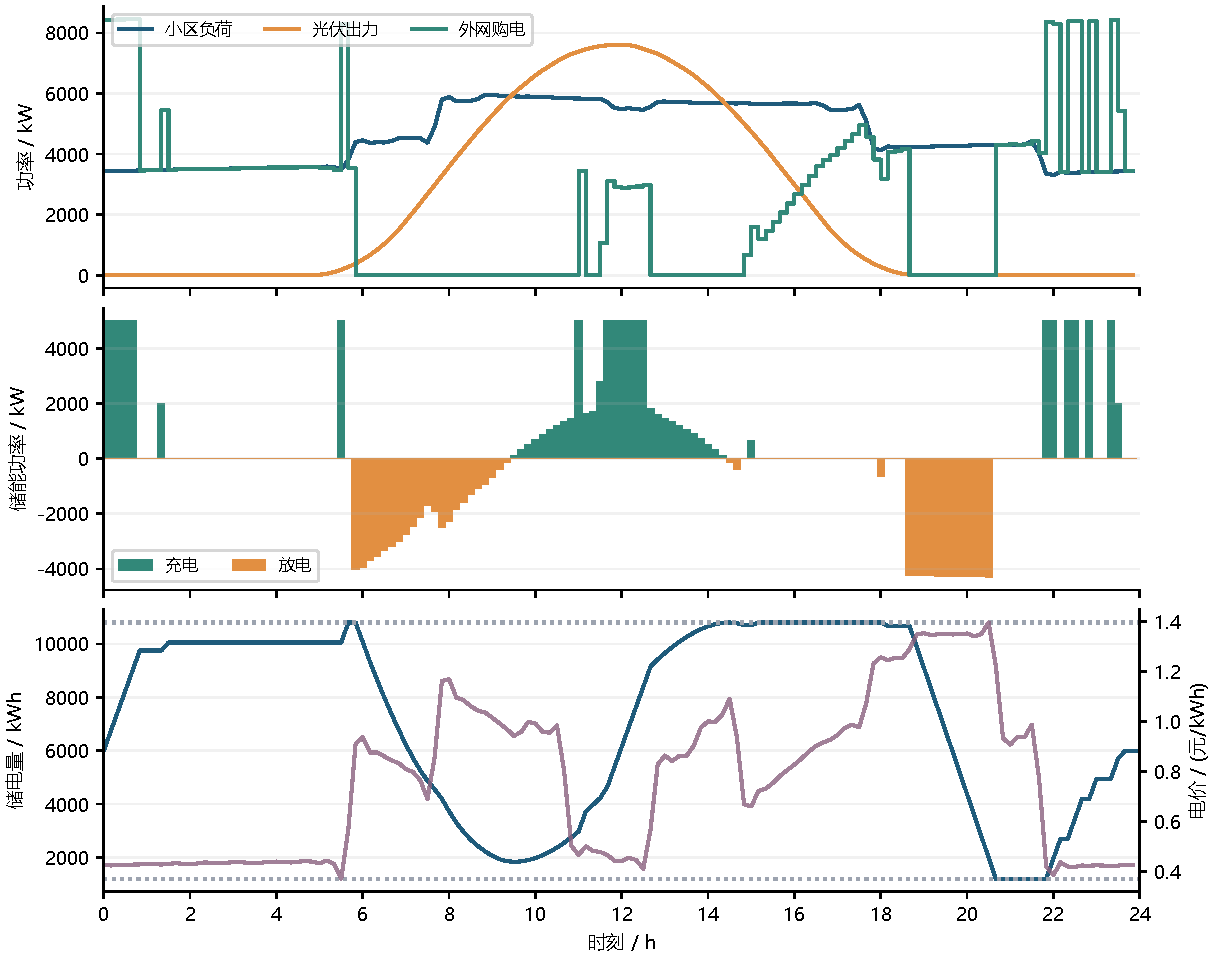
\includegraphics[width=0.94\linewidth]{figures/results/q1_dispatch.pdf}
\caption{问题一购电、充放电、储电量及电价}\label{fig:q1}
\end{figure}
\FloatBarrier

\subsection{问题二：场景采购的经济贡献}

评价期计划费用13507968.43元、紧急费用504839.24元，总费用14012807.66元，紧急购电85017.69 kWh，涉及113天、617个10分钟时段。紧急补购后逐段满足负载；出现紧急购电表示额外昂贵采购，不表示已经发生失供电。

表\ref{tab:v2_baselines}固定同一预测器、执行器及评价期初态。点预测采购费用15290840.75元，无储能场景采购费用18548033.07元。相较点预测，场景期望费用方案节省1278033.08元，即8.36\%；相较无储能场景采购节省24.45\%。主要收益来自对五倍补购的非对称代价进行场景评估，以及电池的跨时段能量转移。该证据支持场景采购，但不意味着必须额外加入风险惩罚。

\begin{table}[htbp]\centering\small
\caption{问题2在相同预测与初态下的基础对照}
\label{tab:v2_baselines}
\begin{tabularx}{\linewidth}{LRRRR}\toprule
策略 & 总费/万元 & 紧急量/kWh & 日费CVaR95/元 & 末库存/kWh\\\midrule
无储能场景采购 & 1854.80 & 242340.86 & 80425.37 & 8875.19\\
点预测采购 & 1529.08 & 505585.75 & 100557.90 & 5845.40\\
场景期望费用（主案） & 1401.28 & 85017.69 & 70731.74 & 6240.32\\
\bottomrule\end{tabularx}
\par\smallskip\parbox{\linewidth}{\footnotesize 所有对照覆盖相同334天；设置在运行前冻结，评价期结果不回写主案选择。各组状态连续演化。}
\end{table}
\begin{table}[htbp]\centering\small
\caption{问题2指定日期购电结果（沿用题目表1布局，电量单位：kWh）}
\label{tab:q2-purchase}
\par\smallskip\textbf{2025-03-20}\par\smallskip
\begin{tabularx}{\linewidth}{lRlRlR}
\toprule
时间段 & 购电量 & 时间段 & 购电量 & 时间段 & 购电量\\
\midrule
10:00--10:10 & 0.00 & 12:00--12:10 & 564.20 & 14:00--14:10 & 0.00\\
16:00--16:10 & 490.32 & 18:00--18:10 & 704.86 & 20:00--20:10 & 0.00\\
\midrule
全天购电量 & 67796.64 & \multicolumn{2}{c}{全天购电费（元）} & \multicolumn{2}{r}{41219.41}\\
\bottomrule
\end{tabularx}
\par\smallskip\textbf{2025-06-21}\par\smallskip
\begin{tabularx}{\linewidth}{lRlRlR}
\toprule
时间段 & 购电量 & 时间段 & 购电量 & 时间段 & 购电量\\
\midrule
10:00--10:10 & 0.00 & 12:00--12:10 & 0.00 & 14:00--14:10 & 0.00\\
16:00--16:10 & 296.43 & 18:00--18:10 & 275.52 & 20:00--20:10 & 0.00\\
\midrule
全天购电量 & 40036.30 & \multicolumn{2}{c}{全天购电费（元）} & \multicolumn{2}{r}{23986.38}\\
\bottomrule
\end{tabularx}
\par\smallskip\textbf{2025-09-23}\par\smallskip
\begin{tabularx}{\linewidth}{lRlRlR}
\toprule
时间段 & 购电量 & 时间段 & 购电量 & 时间段 & 购电量\\
\midrule
10:00--10:10 & 0.00 & 12:00--12:10 & 475.29 & 14:00--14:10 & 0.00\\
16:00--16:10 & 537.29 & 18:00--18:10 & 789.93 & 20:00--20:10 & 0.00\\
\midrule
全天购电量 & 69576.50 & \multicolumn{2}{c}{全天购电费（元）} & \multicolumn{2}{r}{46384.26}\\
\bottomrule
\end{tabularx}
\par\smallskip\textbf{2025-12-21}\par\smallskip
\begin{tabularx}{\linewidth}{lRlRlR}
\toprule
时间段 & 购电量 & 时间段 & 购电量 & 时间段 & 购电量\\
\midrule
10:00--10:10 & 0.00 & 12:00--12:10 & 970.92 & 14:00--14:10 & 0.00\\
16:00--16:10 & 851.12 & 18:00--18:10 & 744.23 & 20:00--20:10 & 0.00\\
\midrule
全天购电量 & 101008.53 & \multicolumn{2}{c}{全天购电费（元）} & \multicolumn{2}{r}{65454.44}\\
\bottomrule
\end{tabularx}
\par\smallskip\parbox{\linewidth}{\footnotesize 注：问题2与4-2列示计划购电量；问题3与4-3列示最终生效的调整后常规购电量。全天购电量不含紧急购电，全天购电费含计划、调整与紧急费用。}
\end{table}

\begin{table}[htbp]\centering\small
\caption{问题2指定日期储能结果（沿用题目表2布局，单位：kWh）}
\label{tab:q2-battery}
\par\smallskip\textbf{2025-03-20}\par\smallskip
\begin{tabularx}{\linewidth}{lRRlRR}
\toprule
时间段 & 充电量 & 放电量 & 时间段 & 充电量 & 放电量\\
\midrule
00:00--04:00 & 3924.13 & 181.53 & 04:00--08:00 & 1015.09 & 5240.21\\
08:00--12:00 & 6123.03 & 2777.38 & 12:00--16:00 & 3923.99 & 420.71\\
16:00--20:00 & 268.54 & 5719.49 & 20:00--24:00 & 5703.85 & 2960.43\\
\midrule
0:00储电量 & \multicolumn{2}{r}{6705.54} & 24:00储电量 & \multicolumn{2}{r}{6346.37}\\
\bottomrule
\end{tabularx}
\par\smallskip\textbf{2025-06-21}\par\smallskip
\begin{tabularx}{\linewidth}{lRRlRR}
\toprule
时间段 & 充电量 & 放电量 & 时间段 & 充电量 & 放电量\\
\midrule
00:00--04:00 & 1394.50 & 465.11 & 04:00--08:00 & 460.19 & 4390.39\\
08:00--12:00 & 6534.90 & 0.00 & 12:00--16:00 & 0.00 & 0.00\\
16:00--20:00 & 156.59 & 4882.20 & 20:00--24:00 & 6792.80 & 2485.90\\
\midrule
0:00储电量 & \multicolumn{2}{r}{8644.37} & 24:00储电量 & \multicolumn{2}{r}{8867.68}\\
\bottomrule
\end{tabularx}
\par\smallskip\textbf{2025-09-23}\par\smallskip
\begin{tabularx}{\linewidth}{lRRlRR}
\toprule
时间段 & 充电量 & 放电量 & 时间段 & 充电量 & 放电量\\
\midrule
00:00--04:00 & 4692.99 & 53.14 & 04:00--08:00 & 916.24 & 5893.48\\
08:00--12:00 & 5977.49 & 1896.62 & 12:00--16:00 & 3708.39 & 625.98\\
16:00--20:00 & 151.78 & 5739.35 & 20:00--24:00 & 5609.40 & 2640.89\\
\midrule
0:00储电量 & \multicolumn{2}{r}{6006.02} & 24:00储电量 & \multicolumn{2}{r}{6235.06}\\
\bottomrule
\end{tabularx}
\par\smallskip\textbf{2025-12-21}\par\smallskip
\begin{tabularx}{\linewidth}{lRRlRR}
\toprule
时间段 & 充电量 & 放电量 & 时间段 & 充电量 & 放电量\\
\midrule
00:00--04:00 & 4499.79 & 40.16 & 04:00--08:00 & 762.27 & 1359.20\\
08:00--12:00 & 5913.75 & 6490.57 & 12:00--16:00 & 5645.48 & 2130.65\\
16:00--20:00 & 0.00 & 5526.27 & 20:00--24:00 & 5771.81 & 2842.53\\
\midrule
0:00储电量 & \multicolumn{2}{r}{6794.81} & 24:00储电量 & \multicolumn{2}{r}{6695.97}\\
\bottomrule
\end{tabularx}
\end{table}

\begin{table}[htbp]\centering\small
\caption{问题2指定日期紧急购电（题目表3布局，单位：kWh）}
\label{tab:q2-emergency}
\setlength{\tabcolsep}{3pt}
\begin{tabularx}{\linewidth}{lRlRlRlR}\toprule
\multicolumn{2}{c}{2025-03-20} & \multicolumn{2}{c}{2025-06-21} & \multicolumn{2}{c}{2025-09-23} & \multicolumn{2}{c}{2025-12-21}\\
时间段 & 购电量 & 时间段 & 购电量 & 时间段 & 购电量 & 时间段 & 购电量\\\midrule
无 & 0.00 & 无 & 0.00 & 20:20--20:40 & 388.40 & 无 & 0.00\\
 &   &  &   & 20:50--21:10 & 90.05 &  &  \\
 &   &  &   & 21:20--21:50 & 34.20 &  &  \\
\midrule
合计 & 0.00 & 合计 & 0.00 & 合计 & 512.64 & 合计 & 0.00\\
\bottomrule\end{tabularx}\end{table}

四个指定日期中，9月23日存在三段紧急购电，合计512.64 kWh，其余三个日期为零。相邻正值时段才合并，夹有零紧急量时保留分段。四小时区间内充、放电量可以同时为正，表示不同10分钟时段各自充电或放电，不违反单时段互斥。
\FloatBarrier

\subsection{问题三：交易修订与反馈来源}

问题三计划费用13674565.95元、调整费用230664.95元、紧急费用70579.96元，总费用13975810.86元。紧急购电12647.76 kWh，涉及92天、282个时段。与问题二相比，费用降低0.2640\%，紧急量降低85.12\%。两问零时光伏信息不同、各自一月末态也不同，因此这一横向差异不是滚动更新本身的独立因果收益。

为区分信息来源，表\ref{tab:v2_feedback}在同一问题三模型下依次比较：仅零时外层计划；6、12、18时仅更新SOC并按零时预测重优化；再加入新发布光伏；最后加入已观测负荷偏差反馈。四组均采用规则执行，不启用跨日候选，因此不会通过续接预测把新信息带入“SOC-only”组。

\begin{table}[htbp]\centering\small
\caption{问题3的状态、光伏和负荷反馈分解}
\label{tab:v2_feedback}
\begin{tabularx}{\linewidth}{LRRRR}\toprule
策略 & 总费/万元 & 紧急量/kWh & 日费CVaR95/元 & 末库存/kWh\\\midrule
仅零时外层计划 & 1416.90 & 80181.62 & 71801.23 & 6240.32\\
仅更新SOC并重优化 & 1399.17 & 39298.96 & 66748.14 & 6240.32\\
再加入新光伏预报 & 1407.57 & 40071.16 & 66732.97 & 6240.32\\
再加入负荷偏差反馈 & 1397.58 & 12647.76 & 65518.79 & 6240.32\\
\bottomrule\end{tabularx}
\par\smallskip\parbox{\linewidth}{\footnotesize 所有对照覆盖相同334天；设置在运行前冻结，评价期结果不回写主案选择。各组状态连续演化。}
\end{table}

仅零时外层计划的费用为14169011.89元，更新SOC并重优化后降至13991697.93元，减少177313.97元；再加入新光伏预报，费用增至14075665.67元；进一步加入负荷偏差反馈，费用降至13975810.86元。新光伏这一增量在本回测中增加83967.74元，随后负荷反馈减少99854.81元。这些是相同设置下的闭环路径差异，体现采购、状态和预测误差相互作用，不能将每份新预报的价值预设为正。所有预报发布时间以外的新预报均未由附件提供，不能用实际未来光伏代替不存在的高频预报来计算收益。

图\ref{fig:v2-control}选取评价期紧急购电量最大日7月4日，以独立纵轴显示上调量、参考与实际SOC、紧急量。清晨实际电量比参考更早触及下限，6时前集中补购；中午参考轨迹因外层重新初始化出现跳变，不能将拼接参考曲线当成一条连续实施轨迹。图\ref{fig:v2-adjustments}另列四个指定日期的调整量，避免计划与最终购电曲线重合掩盖修订幅度。

\begin{figure}[htbp]\centering
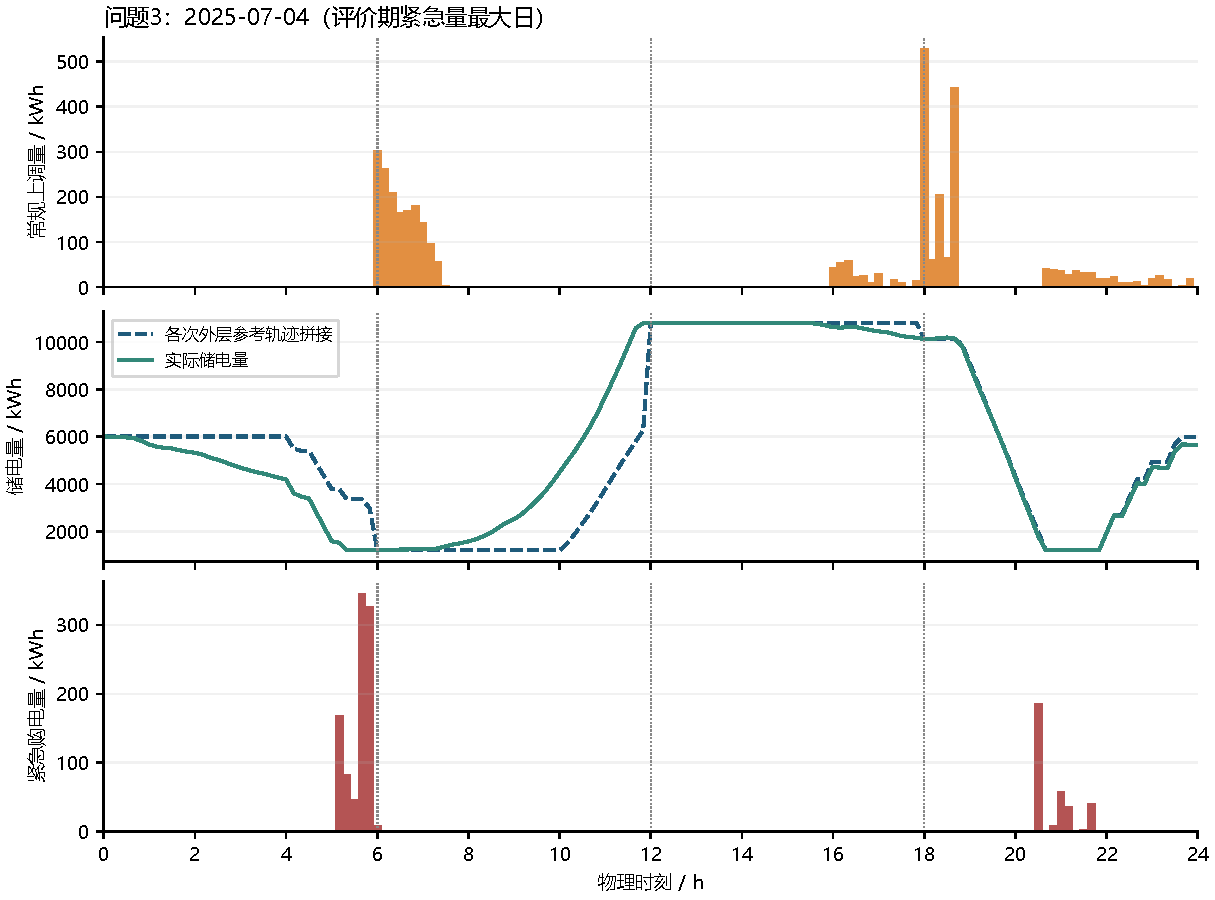
\includegraphics[width=0.96\linewidth]{figures/results/v2_control_difference.pdf}
\caption{问题三紧急量最大日的调整、SOC偏差与紧急购电；虚线标示合法外层修订时点}\label{fig:v2-control}
\end{figure}
\begin{figure}[htbp]\centering
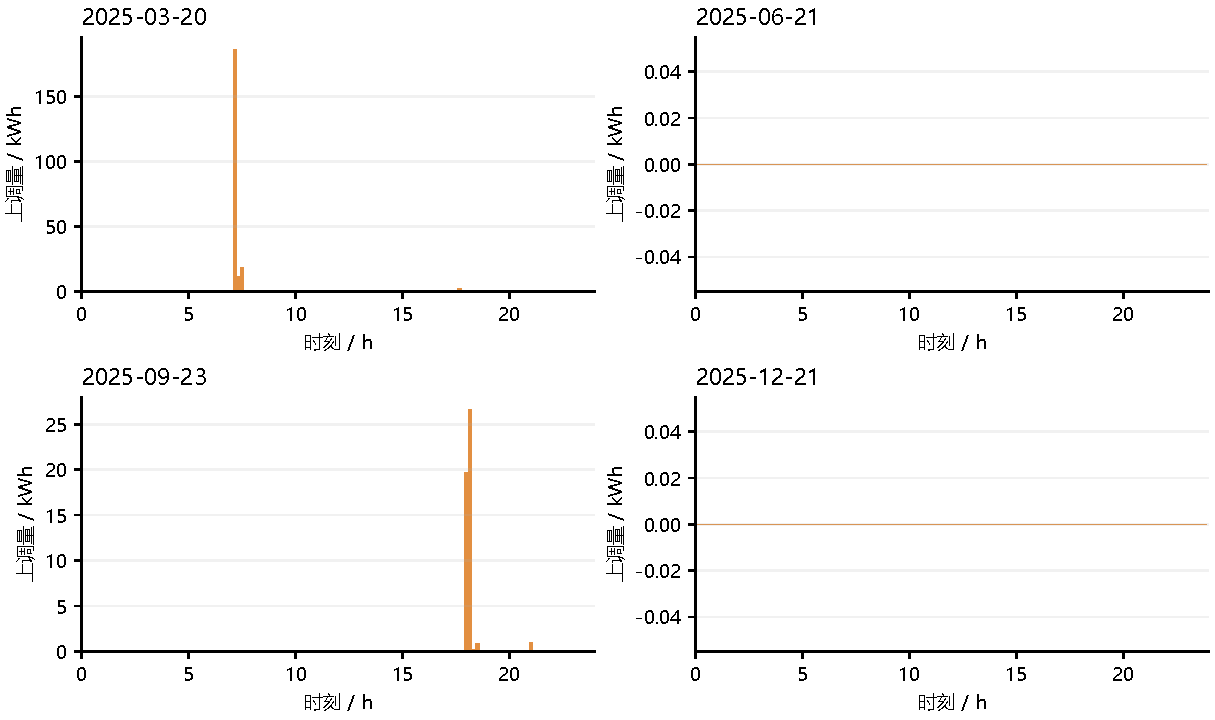
\includegraphics[width=0.96\linewidth]{figures/results/v2_adjustments.pdf}
\caption{四个指定日期的常规购电调整量$a_t-g_t$}\label{fig:v2-adjustments}
\end{figure}
\begin{table}[htbp]\centering\small
\caption{问题3指定日期购电结果（沿用题目表1布局，电量单位：kWh）}
\label{tab:q3-purchase}
\par\smallskip\textbf{2025-03-20}\par\smallskip
\begin{tabularx}{\linewidth}{lRlRlR}
\toprule
时间段 & 购电量 & 时间段 & 购电量 & 时间段 & 购电量\\
\midrule
10:00--10:10 & 0.00 & 12:00--12:10 & 624.29 & 14:00--14:10 & 0.00\\
16:00--16:10 & 671.04 & 18:00--18:10 & 704.20 & 20:00--20:10 & 0.00\\
\midrule
全天购电量 & 71668.03 & \multicolumn{2}{c}{全天购电费（元）} & \multicolumn{2}{r}{45101.87}\\
\bottomrule
\end{tabularx}
\par\smallskip\textbf{2025-06-21}\par\smallskip
\begin{tabularx}{\linewidth}{lRlRlR}
\toprule
时间段 & 购电量 & 时间段 & 购电量 & 时间段 & 购电量\\
\midrule
10:00--10:10 & 0.00 & 12:00--12:10 & 0.00 & 14:00--14:10 & 0.00\\
16:00--16:10 & 298.65 & 18:00--18:10 & 298.84 & 20:00--20:10 & 0.00\\
\midrule
全天购电量 & 38517.86 & \multicolumn{2}{c}{全天购电费（元）} & \multicolumn{2}{r}{23116.13}\\
\bottomrule
\end{tabularx}
\par\smallskip\textbf{2025-09-23}\par\smallskip
\begin{tabularx}{\linewidth}{lRlRlR}
\toprule
时间段 & 购电量 & 时间段 & 购电量 & 时间段 & 购电量\\
\midrule
10:00--10:10 & 0.00 & 12:00--12:10 & 444.81 & 14:00--14:10 & 0.00\\
16:00--16:10 & 611.01 & 18:00--18:10 & 821.01 & 20:00--20:10 & 0.00\\
\midrule
全天购电量 & 73520.35 & \multicolumn{2}{c}{全天购电费（元）} & \multicolumn{2}{r}{46282.76}\\
\bottomrule
\end{tabularx}
\par\smallskip\textbf{2025-12-21}\par\smallskip
\begin{tabularx}{\linewidth}{lRlRlR}
\toprule
时间段 & 购电量 & 时间段 & 购电量 & 时间段 & 购电量\\
\midrule
10:00--10:10 & 0.00 & 12:00--12:10 & 1054.19 & 14:00--14:10 & 0.00\\
16:00--16:10 & 877.48 & 18:00--18:10 & 744.23 & 20:00--20:10 & 0.00\\
\midrule
全天购电量 & 101747.42 & \multicolumn{2}{c}{全天购电费（元）} & \multicolumn{2}{r}{65702.81}\\
\bottomrule
\end{tabularx}
\par\smallskip\parbox{\linewidth}{\footnotesize 注：问题2与4-2列示计划购电量；问题3与4-3列示最终生效的调整后常规购电量。全天购电量不含紧急购电，全天购电费含计划、调整与紧急费用。}
\end{table}

\begin{table}[htbp]\centering\small
\caption{问题3指定日期储能结果（沿用题目表2布局，单位：kWh）}
\label{tab:q3-battery}
\par\smallskip\textbf{2025-03-20}\par\smallskip
\begin{tabularx}{\linewidth}{lRRlRR}
\toprule
时间段 & 充电量 & 放电量 & 时间段 & 充电量 & 放电量\\
\midrule
00:00--04:00 & 3924.11 & 181.53 & 04:00--08:00 & 882.86 & 6102.55\\
08:00--12:00 & 5765.88 & 2564.56 & 12:00--16:00 & 5215.25 & 254.72\\
16:00--20:00 & 1.31 & 5594.70 & 20:00--24:00 & 5703.85 & 2960.43\\
\midrule
0:00储电量 & \multicolumn{2}{r}{6705.56} & 24:00储电量 & \multicolumn{2}{r}{6428.95}\\
\bottomrule
\end{tabularx}
\par\smallskip\textbf{2025-06-21}\par\smallskip
\begin{tabularx}{\linewidth}{lRRlRR}
\toprule
时间段 & 充电量 & 放电量 & 时间段 & 充电量 & 放电量\\
\midrule
00:00--04:00 & 1341.57 & 1491.63 & 04:00--08:00 & 554.21 & 4390.39\\
08:00--12:00 & 7761.12 & 0.00 & 12:00--16:00 & 0.00 & 0.00\\
16:00--20:00 & 127.81 & 4858.89 & 20:00--24:00 & 6792.80 & 2485.90\\
\midrule
0:00储电量 & \multicolumn{2}{r}{8644.37} & 24:00储电量 & \multicolumn{2}{r}{8867.68}\\
\bottomrule
\end{tabularx}
\par\smallskip\textbf{2025-09-23}\par\smallskip
\begin{tabularx}{\linewidth}{lRRlRR}
\toprule
时间段 & 充电量 & 放电量 & 时间段 & 充电量 & 放电量\\
\midrule
00:00--04:00 & 4692.26 & 53.14 & 04:00--08:00 & 892.10 & 5612.58\\
08:00--12:00 & 6293.08 & 1896.62 & 12:00--16:00 & 3282.98 & 403.62\\
16:00--20:00 & 15.07 & 5618.19 & 20:00--24:00 & 5609.40 & 3046.08\\
\midrule
0:00储电量 & \multicolumn{2}{r}{6006.68} & 24:00储电量 & \multicolumn{2}{r}{6235.06}\\
\bottomrule
\end{tabularx}
\par\smallskip\textbf{2025-12-21}\par\smallskip
\begin{tabularx}{\linewidth}{lRRlRR}
\toprule
时间段 & 充电量 & 放电量 & 时间段 & 充电量 & 放电量\\
\midrule
00:00--04:00 & 4496.41 & 40.16 & 04:00--08:00 & 762.28 & 1406.28\\
08:00--12:00 & 6441.76 & 6526.43 & 12:00--16:00 & 5333.82 & 2222.97\\
16:00--20:00 & 0.00 & 5526.27 & 20:00--24:00 & 5771.81 & 2842.53\\
\midrule
0:00储电量 & \multicolumn{2}{r}{6797.85} & 24:00储电量 & \multicolumn{2}{r}{6695.97}\\
\bottomrule
\end{tabularx}
\end{table}

\begin{table}[htbp]\centering\small
\caption{问题3指定日期紧急购电（题目表3布局，单位：kWh）}
\label{tab:q3-emergency}
\setlength{\tabcolsep}{3pt}
\begin{tabularx}{\linewidth}{lRlRlRlR}\toprule
\multicolumn{2}{c}{2025-03-20} & \multicolumn{2}{c}{2025-06-21} & \multicolumn{2}{c}{2025-09-23} & \multicolumn{2}{c}{2025-12-21}\\
时间段 & 购电量 & 时间段 & 购电量 & 时间段 & 购电量 & 时间段 & 购电量\\\midrule
09:10--10:00 & 212.82 & 无 & 0.00 & 20:20--20:30 & 6.38 & 无 & 0.00\\
 &   &  &   & 20:50--21:10 & 65.84 &  &  \\
 &   &  &   & 21:20--21:50 & 34.20 &  &  \\
\midrule
合计 & 212.82 & 合计 & 0.00 & 合计 & 106.42 & 合计 & 0.00\\
\bottomrule\end{tabularx}\end{table}
\FloatBarrier

\subsection{问题四：联合价格不确定下的采购与滚动调度}

动态电价下静态方案计划费用14280142.03元、紧急费用513982.26元，总费用14794124.29元，紧急电量80544.00 kWh。滚动方案计划费用14460229.83元、调整费用241942.19元、紧急费用67060.51元，总费用14769232.53元，紧急电量11950.68 kWh。两案费用相差24891.76元，即0.1683\%，而紧急电量降低85.16\%。

这一结果说明昂贵补购减少并不必然带来同比例的总费用下降：增加常规承诺和修订仍须付款。滚动案实际日费用CVaR95为77420.84元，静态案为83044.31元；它们是已实现账单的描述，不是风险扩展效果的证明。本节两案的预测配置和期初库存也有所区别，费用差不能全部归为单个价格预测或控制模块。

联合场景采用同日价荷残差，依据价格加权分位数的机制解释，高缺口是否伴随高电价会影响采购。有限历史窗口并不能覆盖所有价荷状态，不能把单时段80\%分位数直接用作含储能系统的逐时公式。四个指定日期的常规采购、储能与紧急结果如下，具体计划费与调整费分解附于支撑表。

\begin{table}[htbp]\centering\small
\caption{问题4-2指定日期购电结果（沿用题目表1布局，电量单位：kWh）}
\label{tab:q4_2-purchase}
\par\smallskip\textbf{2025-03-20}\par\smallskip
\begin{tabularx}{\linewidth}{lRlRlR}
\toprule
时间段 & 购电量 & 时间段 & 购电量 & 时间段 & 购电量\\
\midrule
10:00--10:10 & 0.00 & 12:00--12:10 & 564.20 & 14:00--14:10 & 0.00\\
16:00--16:10 & 490.32 & 18:00--18:10 & 0.00 & 20:00--20:10 & 743.27\\
\midrule
全天购电量 & 67869.67 & \multicolumn{2}{c}{全天购电费（元）} & \multicolumn{2}{r}{42207.16}\\
\bottomrule
\end{tabularx}
\par\smallskip\textbf{2025-06-21}\par\smallskip
\begin{tabularx}{\linewidth}{lRlRlR}
\toprule
时间段 & 购电量 & 时间段 & 购电量 & 时间段 & 购电量\\
\midrule
10:00--10:10 & 0.00 & 12:00--12:10 & 0.00 & 14:00--14:10 & 0.00\\
16:00--16:10 & 296.43 & 18:00--18:10 & 510.07 & 20:00--20:10 & 0.00\\
\midrule
全天购电量 & 40675.72 & \multicolumn{2}{c}{全天购电费（元）} & \multicolumn{2}{r}{21012.94}\\
\bottomrule
\end{tabularx}
\par\smallskip\textbf{2025-09-23}\par\smallskip
\begin{tabularx}{\linewidth}{lRlRlR}
\toprule
时间段 & 购电量 & 时间段 & 购电量 & 时间段 & 购电量\\
\midrule
10:00--10:10 & 0.00 & 12:00--12:10 & 497.24 & 14:00--14:10 & 0.00\\
16:00--16:10 & 537.29 & 18:00--18:10 & 0.00 & 20:00--20:10 & 0.00\\
\midrule
全天购电量 & 69762.68 & \multicolumn{2}{c}{全天购电费（元）} & \multicolumn{2}{r}{48309.88}\\
\bottomrule
\end{tabularx}
\par\smallskip\textbf{2025-12-21}\par\smallskip
\begin{tabularx}{\linewidth}{lRlRlR}
\toprule
时间段 & 购电量 & 时间段 & 购电量 & 时间段 & 购电量\\
\midrule
10:00--10:10 & 0.00 & 12:00--12:10 & 970.92 & 14:00--14:10 & 0.00\\
16:00--16:10 & 851.12 & 18:00--18:10 & 744.23 & 20:00--20:10 & 0.00\\
\midrule
全天购电量 & 100945.95 & \multicolumn{2}{c}{全天购电费（元）} & \multicolumn{2}{r}{77020.40}\\
\bottomrule
\end{tabularx}
\par\smallskip\parbox{\linewidth}{\footnotesize 注：问题2与4-2列示计划购电量；问题3与4-3列示最终生效的调整后常规购电量。全天购电量不含紧急购电，全天购电费含计划、调整与紧急费用。}
\end{table}

\begin{table}[htbp]\centering\small
\caption{问题4-2指定日期储能结果（沿用题目表2布局，单位：kWh）}
\label{tab:q4_2-battery}
\par\smallskip\textbf{2025-03-20}\par\smallskip
\begin{tabularx}{\linewidth}{lRRlRR}
\toprule
时间段 & 充电量 & 放电量 & 时间段 & 充电量 & 放电量\\
\midrule
00:00--04:00 & 3824.42 & 134.84 & 04:00--08:00 & 1669.83 & 5857.47\\
08:00--12:00 & 6146.04 & 2777.38 & 12:00--16:00 & 3907.13 & 420.71\\
16:00--20:00 & 174.78 & 6369.00 & 20:00--24:00 & 5798.62 & 2212.03\\
\midrule
0:00储电量 & \multicolumn{2}{r}{6834.43} & 24:00储电量 & \multicolumn{2}{r}{6457.15}\\
\bottomrule
\end{tabularx}
\par\smallskip\textbf{2025-06-21}\par\smallskip
\begin{tabularx}{\linewidth}{lRRlRR}
\toprule
时间段 & 充电量 & 放电量 & 时间段 & 充电量 & 放电量\\
\midrule
00:00--04:00 & 963.51 & 3780.66 & 04:00--08:00 & 1400.69 & 1719.95\\
08:00--12:00 & 6932.04 & 0.00 & 12:00--16:00 & 0.00 & 0.00\\
16:00--20:00 & 0.00 & 4853.45 & 20:00--24:00 & 7501.98 & 3091.92\\
\midrule
0:00储电量 & \multicolumn{2}{r}{8545.17} & 24:00储电量 & \multicolumn{2}{r}{8723.59}\\
\bottomrule
\end{tabularx}
\par\smallskip\textbf{2025-09-23}\par\smallskip
\begin{tabularx}{\linewidth}{lRRlRR}
\toprule
时间段 & 充电量 & 放电量 & 时间段 & 充电量 & 放电量\\
\midrule
00:00--04:00 & 5330.27 & 22.20 & 04:00--08:00 & 206.94 & 5820.07\\
08:00--12:00 & 5946.19 & 1896.62 & 12:00--16:00 & 3587.87 & 530.87\\
16:00--20:00 & 163.52 & 6562.31 & 20:00--24:00 & 5525.15 & 1842.66\\
\midrule
0:00储电量 & \multicolumn{2}{r}{6002.76} & 24:00储电量 & \multicolumn{2}{r}{6159.23}\\
\bottomrule
\end{tabularx}
\par\smallskip\textbf{2025-12-21}\par\smallskip
\begin{tabularx}{\linewidth}{lRRlRR}
\toprule
时间段 & 充电量 & 放电量 & 时间段 & 充电量 & 放电量\\
\midrule
00:00--04:00 & 4499.29 & 40.16 & 04:00--08:00 & 0.00 & 741.76\\
08:00--12:00 & 5940.70 & 6486.91 & 12:00--16:00 & 5724.46 & 2220.11\\
16:00--20:00 & 0.00 & 5500.96 & 20:00--24:00 & 5818.48 & 2842.53\\
\midrule
0:00储电量 & \multicolumn{2}{r}{6795.26} & 24:00储电量 & \multicolumn{2}{r}{6766.10}\\
\bottomrule
\end{tabularx}
\end{table}

\begin{table}[htbp]\centering\small
\caption{问题4-2指定日期紧急购电（题目表3布局，单位：kWh）}
\label{tab:q4_2-emergency}
\setlength{\tabcolsep}{3pt}
\begin{tabularx}{\linewidth}{lRlRlRlR}\toprule
\multicolumn{2}{c}{2025-03-20} & \multicolumn{2}{c}{2025-06-21} & \multicolumn{2}{c}{2025-09-23} & \multicolumn{2}{c}{2025-12-21}\\
时间段 & 购电量 & 时间段 & 购电量 & 时间段 & 购电量 & 时间段 & 购电量\\\midrule
无 & 0.00 & 无 & 0.00 & 18:20--18:40 & 3.91 & 无 & 0.00\\
 &   &  &   & 20:30--20:40 & 357.19 &  &  \\
 &   &  &   & 20:50--21:10 & 90.05 &  &  \\
 &   &  &   & 21:20--21:50 & 34.20 &  &  \\
\midrule
合计 & 0.00 & 合计 & 0.00 & 合计 & 485.35 & 合计 & 0.00\\
\bottomrule\end{tabularx}\end{table}
\FloatBarrier
\begin{table}[htbp]\centering\small
\caption{问题4-3指定日期购电结果（沿用题目表1布局，电量单位：kWh）}
\label{tab:q4_3-purchase}
\par\smallskip\textbf{2025-03-20}\par\smallskip
\begin{tabularx}{\linewidth}{lRlRlR}
\toprule
时间段 & 购电量 & 时间段 & 购电量 & 时间段 & 购电量\\
\midrule
10:00--10:10 & 0.00 & 12:00--12:10 & 624.29 & 14:00--14:10 & 0.00\\
16:00--16:10 & 671.04 & 18:00--18:10 & 704.20 & 20:00--20:10 & 743.27\\
\midrule
全天购电量 & 71207.11 & \multicolumn{2}{c}{全天购电费（元）} & \multicolumn{2}{r}{44953.28}\\
\bottomrule
\end{tabularx}
\par\smallskip\textbf{2025-06-21}\par\smallskip
\begin{tabularx}{\linewidth}{lRlRlR}
\toprule
时间段 & 购电量 & 时间段 & 购电量 & 时间段 & 购电量\\
\midrule
10:00--10:10 & 0.00 & 12:00--12:10 & 0.00 & 14:00--14:10 & 0.00\\
16:00--16:10 & 298.65 & 18:00--18:10 & 527.79 & 20:00--20:10 & 0.00\\
\midrule
全天购电量 & 38859.78 & \multicolumn{2}{c}{全天购电费（元）} & \multicolumn{2}{r}{20404.16}\\
\bottomrule
\end{tabularx}
\par\smallskip\textbf{2025-09-23}\par\smallskip
\begin{tabularx}{\linewidth}{lRlRlR}
\toprule
时间段 & 购电量 & 时间段 & 购电量 & 时间段 & 购电量\\
\midrule
10:00--10:10 & 22.75 & 12:00--12:10 & 461.07 & 14:00--14:10 & 54.35\\
16:00--16:10 & 611.01 & 18:00--18:10 & 0.00 & 20:00--20:10 & 822.11\\
\midrule
全天购电量 & 73220.72 & \multicolumn{2}{c}{全天购电费（元）} & \multicolumn{2}{r}{47794.31}\\
\bottomrule
\end{tabularx}
\par\smallskip\textbf{2025-12-21}\par\smallskip
\begin{tabularx}{\linewidth}{lRlRlR}
\toprule
时间段 & 购电量 & 时间段 & 购电量 & 时间段 & 购电量\\
\midrule
10:00--10:10 & 0.00 & 12:00--12:10 & 1054.19 & 14:00--14:10 & 0.00\\
16:00--16:10 & 877.48 & 18:00--18:10 & 744.23 & 20:00--20:10 & 0.00\\
\midrule
全天购电量 & 101918.89 & \multicolumn{2}{c}{全天购电费（元）} & \multicolumn{2}{r}{77624.69}\\
\bottomrule
\end{tabularx}
\par\smallskip\parbox{\linewidth}{\footnotesize 注：问题2与4-2列示计划购电量；问题3与4-3列示最终生效的调整后常规购电量。全天购电量不含紧急购电，全天购电费含计划、调整与紧急费用。}
\end{table}

\begin{table}[htbp]\centering\small
\caption{问题4-3指定日期储能结果（沿用题目表2布局，单位：kWh）}
\label{tab:q4_3-battery}
\par\smallskip\textbf{2025-03-20}\par\smallskip
\begin{tabularx}{\linewidth}{lRRlRR}
\toprule
时间段 & 充电量 & 放电量 & 时间段 & 充电量 & 放电量\\
\midrule
00:00--04:00 & 3749.67 & 134.84 & 04:00--08:00 & 825.23 & 5868.37\\
08:00--12:00 & 5765.88 & 2777.38 & 12:00--16:00 & 5187.95 & 254.72\\
16:00--20:00 & 28.20 & 6553.40 & 20:00--24:00 & 5792.33 & 1970.23\\
\midrule
0:00储电量 & \multicolumn{2}{r}{6863.37} & 24:00储电量 & \multicolumn{2}{r}{6567.77}\\
\bottomrule
\end{tabularx}
\par\smallskip\textbf{2025-06-21}\par\smallskip
\begin{tabularx}{\linewidth}{lRRlRR}
\toprule
时间段 & 充电量 & 放电量 & 时间段 & 充电量 & 放电量\\
\midrule
00:00--04:00 & 963.73 & 4615.43 & 04:00--08:00 & 1483.09 & 1719.95\\
08:00--12:00 & 7782.82 & 0.00 & 12:00--16:00 & 0.00 & 0.00\\
16:00--20:00 & 0.00 & 4831.44 & 20:00--24:00 & 6954.86 & 2485.90\\
\midrule
0:00储电量 & \multicolumn{2}{r}{8632.64} & 24:00储电量 & \multicolumn{2}{r}{8929.00}\\
\bottomrule
\end{tabularx}
\par\smallskip\textbf{2025-09-23}\par\smallskip
\begin{tabularx}{\linewidth}{lRRlRR}
\toprule
时间段 & 充电量 & 放电量 & 时间段 & 充电量 & 放电量\\
\midrule
00:00--04:00 & 4961.74 & 22.20 & 04:00--08:00 & 177.31 & 5680.26\\
08:00--12:00 & 6536.73 & 1893.23 & 12:00--16:00 & 3099.44 & 353.23\\
16:00--20:00 & 96.08 & 6443.21 & 20:00--24:00 & 5603.57 & 2259.51\\
\midrule
0:00储电量 & \multicolumn{2}{r}{6334.43} & 24:00储电量 & \multicolumn{2}{r}{6260.00}\\
\bottomrule
\end{tabularx}
\par\smallskip\textbf{2025-12-21}\par\smallskip
\begin{tabularx}{\linewidth}{lRRlRR}
\toprule
时间段 & 充电量 & 放电量 & 时间段 & 充电量 & 放电量\\
\midrule
00:00--04:00 & 4436.14 & 40.16 & 04:00--08:00 & 735.70 & 1384.74\\
08:00--12:00 & 6412.06 & 6391.52 & 12:00--16:00 & 5218.63 & 2240.52\\
16:00--20:00 & 0.00 & 5490.42 & 20:00--24:00 & 5769.36 & 2842.53\\
\midrule
0:00储电量 & \multicolumn{2}{r}{6852.09} & 24:00储电量 & \multicolumn{2}{r}{6733.60}\\
\bottomrule
\end{tabularx}
\end{table}

\begin{table}[htbp]\centering\small
\caption{问题4-3指定日期紧急购电（题目表3布局，单位：kWh）}
\label{tab:q4_3-emergency}
\setlength{\tabcolsep}{3pt}
\begin{tabularx}{\linewidth}{lRlRlRlR}\toprule
\multicolumn{2}{c}{2025-03-20} & \multicolumn{2}{c}{2025-06-21} & \multicolumn{2}{c}{2025-09-23} & \multicolumn{2}{c}{2025-12-21}\\
时间段 & 购电量 & 时间段 & 购电量 & 时间段 & 购电量 & 时间段 & 购电量\\\midrule
无 & 0.00 & 无 & 0.00 & 18:30--18:40 & 2.38 & 无 & 0.00\\
 &   &  &   & 20:10--20:20 & 10.23 &  &  \\
\midrule
合计 & 0.00 & 合计 & 0.00 & 合计 & 12.61 & 合计 & 0.00\\
\bottomrule\end{tabularx}\end{table}
\FloatBarrier
\begin{figure}[htbp]\centering
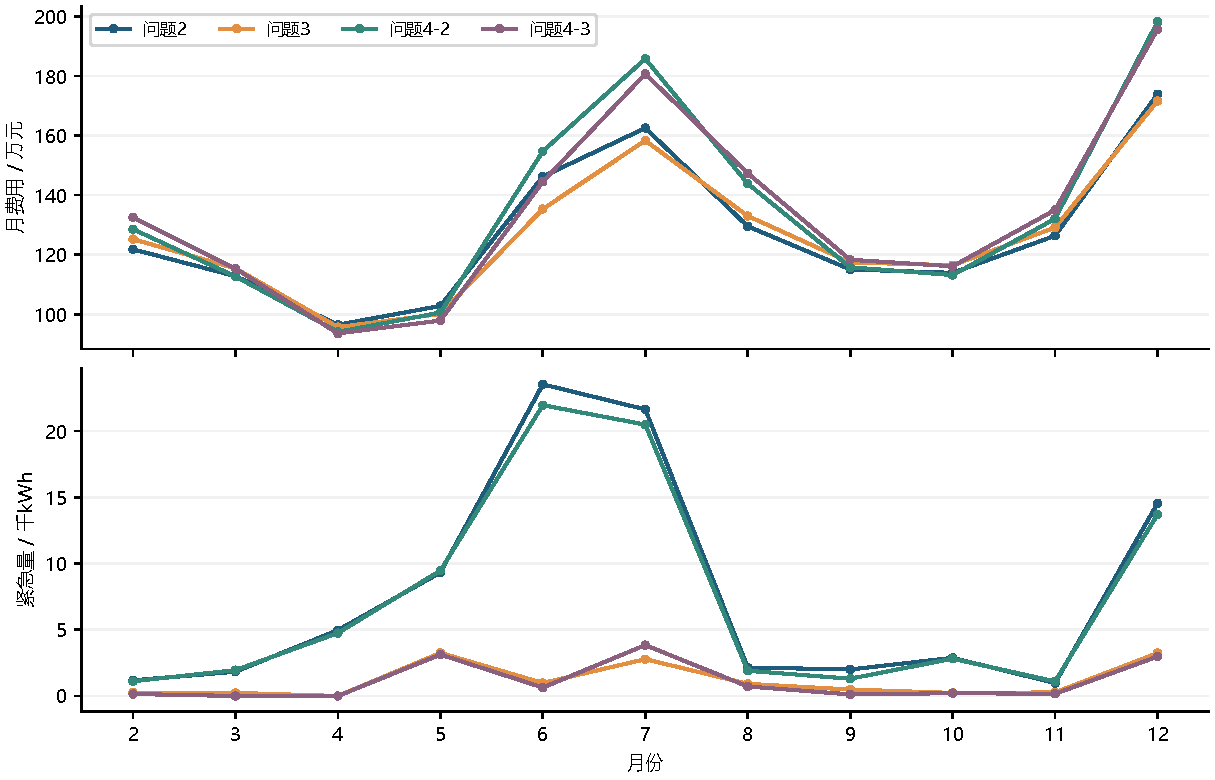
\includegraphics[width=0.95\linewidth]{figures/results/v2_monthly.pdf}
\caption{四组冻结主方案的月度实际费用与紧急购电量}\label{fig:v2-monthly}
\end{figure}

\section{机制检验与扩展策略比较}

\subsection{规划与执行偏差：一致性不等于低费用}

先固定原版参数，即12代表场景、自适应风险基数0.1及参考备用系数1，重建每个外层决策点的购电计划，再将相同历史场景输入原执行规则。重建购电量与保存轨迹在实际执行窗口完全一致。表\ref{tab:v2_execution_gap}汇总2月至12月决策点：问题二、三、四静态和四滚动的平均费用偏差分别为$-986.50$、$-569.90$、$-1068.47$和$-582.32$元，多数回放费用低于规划费用。

\begin{table}[htbp]\centering\small
\caption{原版同计划、同初态、同场景的规划与执行偏差}
\label{tab:v2_execution_gap}
\begin{tabularx}{\linewidth}{LRRRR}\toprule
问题 & 决策点数 & 平均$\Delta_{\rm exec}$/元 & 负偏差比例 & SOC均方根偏差/kWh\\\midrule
问题2 & 334 & -986.50 & 97.90\% & 1319.72\\
问题3 & 1336 & -569.90 & 94.24\% & 994.32\\
问题4-2 & 334 & -1068.47 & 99.40\% & 1350.69\\
问题4-3 & 1336 & -582.32 & 93.94\% & 1048.30\\
\bottomrule\end{tabularx}
\par\smallskip\parbox{\linewidth}{\footnotesize 每一决策点先按场景概率计算费用差与SOC均方根偏差，再对决策点取均值；滚动剩余时域相互重叠，不将这些差求和解释为年度费用。全部费用仅计实际结算项目。}
\end{table}

负偏差不表示规划正确描述了控制，而是参考储能在各场景共享，实际规则可利用当期观测调整动作，其实现费用可能更低。正偏差仍会出现。图\ref{fig:v2-gap}选取问题三正偏差最大决策点，展示不同场景下SOC偏离与费用差发生的时段。两条期望费用都仅计真实收费，不混入风险项或终端罚项；滚动剩余时域相互重叠，不能将这些偏差相加为年度节费。

\begin{figure}[htbp]\centering
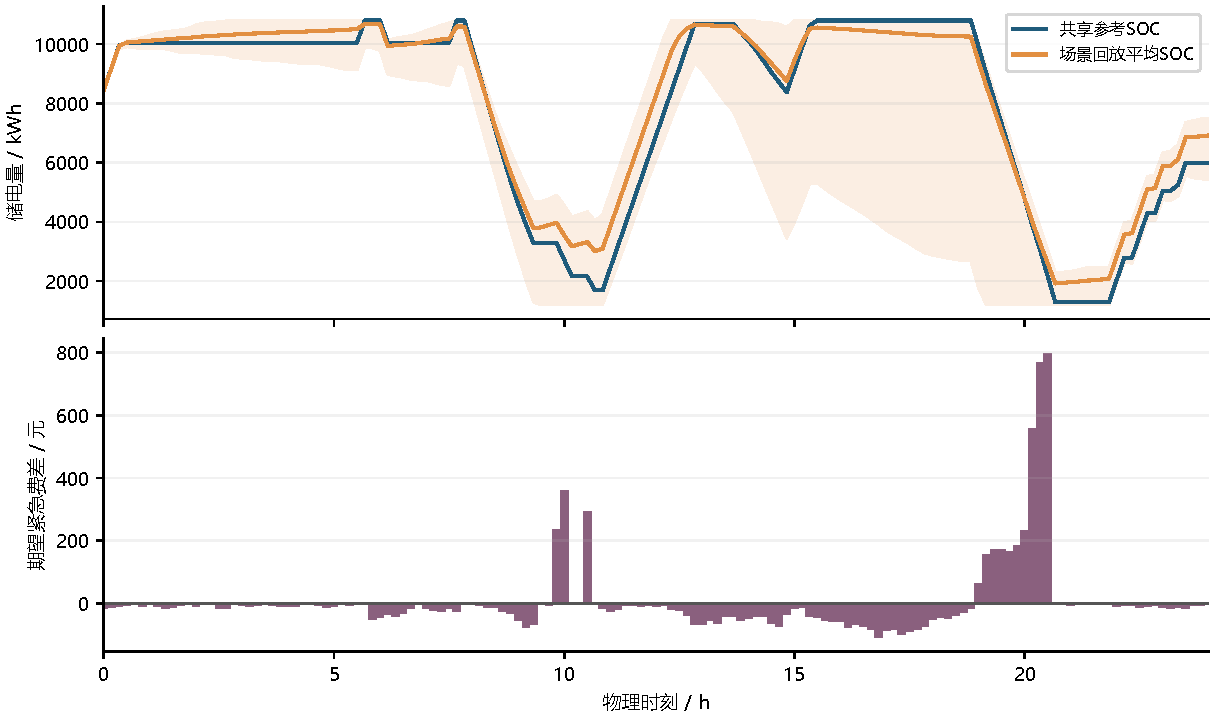
\includegraphics[width=0.96\linewidth]{figures/results/v2_execution_gap.pdf}
\caption{原版问题三正费用偏差最大决策点的参考与场景回放；阴影为回放SOC范围，费用差取回放减规划}\label{fig:v2-gap}
\end{figure}

进一步使用本次冻结的主案，在四个指定日的四个外层时点固定合同、初态及28场景，对规则执行和内层LP各回放448条轨迹。未来输入保持当时合法点预测，只有当前一步揭示场景净需求和价格，不读取未来场景实现或后续新预报。这样把“同计划下换控制器”的影响与“闭环运行导致后来计划也改变”的影响区分开来。

\begin{table}[htbp]\centering\small
\caption{修订主计划下两种执行器的同场景回放诊断}
\label{tab:v2_inner_gap}
\begin{tabularx}{\linewidth}{LRR}\toprule
指标 & 规则执行 & 内层LP\\\midrule
有符号期望费用偏差/元 & -655.33 & -513.41\\
场景费用绝对偏差的期望/元 & 697.25 & 605.16\\
SOC均方根偏差/kWh & 1056.40 & 869.79\\
\bottomrule\end{tabularx}
\par\smallskip\parbox{\linewidth}{\footnotesize 四个指定日、四个时点共16个决策点，每点28场景。先计算场景概率加权指标，再对决策点等权平均；两种执行器固定相同购电合同和初态，仅逐步揭示当前场景值。}
\end{table}

内层LP将SOC均方根偏差均值由1056.40 kWh降至869.79 kWh，场景费用绝对偏差的期望由697.25元降至605.16元；但平均账单相对规则执行增加141.92元。16点中，绝对期望费用偏差在10点减小，实际回放账单仅1点更低。因而更接近参考轨迹是一项可观测改善，却不能替代经济目标。主案继续使用一月选中的执行规则，也承认其与上层场景评估尚未严格一致。

\subsection{风险与备用的单独贡献和联合作用}

题目已通过五倍补购价格计入应急代价，不另外要求紧急量达到某个阈值。表\ref{tab:v2_risk_modules}将期望费用、仅风险、仅备用及二者联合全部列出，风险与备用各比较固定和自适应版本。固定风险权重为一月匹配值0.10368，固定备用为208.67 kWh；二者都不根据评价期结果重新设定。

\begin{table}[htbp]\centering\small
\caption{问题2风险与备用的完整对照}
\label{tab:v2_risk_modules}
\begin{tabularx}{\linewidth}{LRRRR}\toprule
策略 & 总费/万元 & 紧急量/kWh & 日费CVaR95/元 & 末库存/kWh\\\midrule
期望费用 & 1401.28 & 85017.69 & 70731.74 & 6240.32\\
固定风险 & 1411.84 & 56316.17 & 69028.62 & 6318.65\\
自适应风险 & 1405.41 & 66920.81 & 69476.71 & 6255.33\\
固定备用 & 1401.09 & 74987.90 & 70409.51 & 6240.32\\
动态备用 & 1402.30 & 76168.28 & 70299.39 & 6245.11\\
固定风险+备用 & 1413.36 & 49102.47 & 68862.93 & 6318.65\\
自适应风险+备用 & 1406.93 & 59081.98 & 69070.96 & 6260.12\\
自适应联合，12场景 & 1404.26 & 75336.25 & 70065.84 & 6289.57\\
\bottomrule\end{tabularx}
\par\smallskip\parbox{\linewidth}{\footnotesize 所有对照覆盖相同334天；设置在运行前冻结，评价期结果不回写主案选择。各组状态连续演化。}
\end{table}
\begin{table}[htbp]\centering\small
\caption{固定与自适应策略在评价期实现的平均保守程度}
\label{tab:v2_conservatism}
\begin{tabularx}{\linewidth}{LRR}\toprule
策略 & 平均风险权重 & 平均参考备用/kWh\\\midrule
固定风险 & 0.10368 & 0.00\\
自适应风险 & 0.05506 & 0.00\\
固定备用 & 0.00000 & 207.22\\
动态备用 & 0.00000 & 244.39\\
固定联合 & 0.10368 & 207.22\\
自适应联合 & 0.05506 & 244.39\\
\bottomrule\end{tabularx}
\par\smallskip\parbox{\linewidth}{\footnotesize 固定参数由一月动态序列的均值匹配；由于季节与误差分布变化，评价期均值不保证相等，不用评价期重新匹配。}
\end{table}

问题二仅加固定风险或自适应风险分别多支付105631.25元和41280.51元，紧急量分别由85017.69 kWh降至56316.17和66920.81 kWh。固定备用单独使用节省1891.73元，动态备用单独使用增加10152.11元，效果并不统一。联合自适应策略比期望费用主案增加56524.93元，同时紧急量降至59081.98 kWh。这里控制的CVaR损失为紧急费用，实际日总费用尾部另列，不将两个对象混称。

固定与自适应之间的比较应结合平均保守程度。匹配在一月完成，评价期实际平均风险权重分别为0.103681与0.055059，参考备用分别为207.22与244.39 kWh，并未保持相等，故不能把全部费用差解释为“自适应识别风险的能力”。描述性联合交互项定义为$C_{\rm joint}-C_{\rm risk}-C_{\rm reserve}+C_{\rm expectation}$，固定及自适应两组分别为17088.03元和5092.30元。其为正表明本回测中联合使用比两项单独费用变化的线性叠加更贵，但这不是独立因果效应估计，也不是所有参数下都会重复保守的定理。

不以评价期最低费用的固定备用策略替换主案。风险控制回答的是“为减少昂贵补购或特定尾部损失，是否愿意支付额外费用”，应作为运行偏好扩展，而非赛题经济目标自动要求的内容。

\subsection{28日完整场景与12个代表场景}

28个等权历史日的10\%尾部仅有2.8条日轨迹的概率质量，少量样本已使CVaR估计不稳定。压缩成12个带权代表场景又可能把尾部集中到个别代表日。不能仅因两种场景数得出的总费用接近，就认定极端补购的形状也被保留。

\begin{table}[htbp]\centering\small
\caption{历史场景保留与缩减的经济对照}
\label{tab:v2_scenarios}
\begin{tabularx}{\linewidth}{LRRRR}\toprule
策略 & 总费/万元 & 紧急量/kWh & 日费CVaR95/元 & 末库存/kWh\\\midrule
问题2：28场景 & 1401.28 & 85017.69 & 70731.74 & 6240.32\\
问题2：12场景 & 1400.63 & 105407.24 & 72139.66 & 6257.26\\
问题3：28场景 & 1397.58 & 12647.76 & 65518.79 & 6240.32\\
问题3：12场景 & 1393.37 & 16150.68 & 65554.27 & 6271.05\\
\bottomrule\end{tabularx}
\par\smallskip\parbox{\linewidth}{\footnotesize 所有对照覆盖相同334天；设置在运行前冻结，评价期结果不回写主案选择。各组状态连续演化。}
\end{table}
\begin{table}[htbp]\centering\small
\caption{场景规模与每日平均运行时间}
\label{tab:v2_solve_times}
\begin{tabularx}{\linewidth}{LRR}\toprule
问题 & 场景数 & 秒/日\\\midrule
问题2 & 12 & 0.0276\\
问题2 & 28 & 0.0521\\
问题3 & 12 & 0.0699\\
问题3 & 28 & 0.1236\\
\bottomrule\end{tabularx}
\par\smallskip\parbox{\linewidth}{\footnotesize 运行时间含预测、外层求解与执行等开销，并行运行下的本机计时仅供工程量级参考。}
\end{table}

经济目标下，问题二12场景比28场景少付6465.72元，却多用20389.55 kWh紧急电量；问题三少付42065.07元，多用3502.93 kWh紧急电量。自适应风险与备用联合开启时，12场景费用14042623.21元、紧急量75336.25 kWh，28场景费用14069332.59元、紧急量59081.98 kWh，压缩对应的尾部账单与紧急需求发生明显变化。保留28场景没有保证评价期账单最小，但排除了额外的代表日压缩，其运行耗时仍适合本题规模，故按预定设置保留。28日历史本身的样本有限性仍然存在。

\subsection{储能LP和跨日价值的效果与边界}

\begin{table}[htbp]\centering\small
\caption{问题3执行控制与跨日续接对照}
\label{tab:v2_controllers}
\begin{tabularx}{\linewidth}{LRRRR}\toprule
策略 & 总费/万元 & 紧急量/kWh & 日费CVaR95/元 & 末库存/kWh\\\midrule
规则执行（主案） & 1397.58 & 12647.76 & 65518.79 & 6240.32\\
剩余日储能LP & 1421.32 & 23825.27 & 66397.37 & 5934.55\\
储能LP+跨日价值 & 1405.26 & 22407.53 & 66033.05 & 6240.32\\
\bottomrule\end{tabularx}
\par\smallskip\parbox{\linewidth}{\footnotesize 所有对照覆盖相同334天；设置在运行前冻结，评价期结果不回写主案选择。各组状态连续演化。}
\end{table}

在完整闭环对照中，仅将问题三执行器改为剩余日LP，总费用为14213193.28元，比主案增加237382.42元，紧急量也增至23825.27 kWh。该结果与一月选型方向一致，不能为了形成“双时间尺度LP”的亮点而强行将其设为主方案。上层目标仍使用共享参考储能，内层仅依据有限预测近似后续价值，两者组合未必实现更低费用。

对相同LP控制器利用合法跨日预报后，总费用降至14052638.61元，比午夜截断的LP节省160554.67元，紧急量减少1417.74 kWh，年末库存还增加305.77 kWh，说明跨日信息改善并非通过更多放空电池取得。但它仍比规则主案多付76827.75元，不能据此宣称已经成为经济最优策略。

一个两时段例子说明内层LP的经济机制：电池具有1 kWh可对外输出的电量，两段常规合同均为0、净需求均为1 kWh，交易价格分别为1和2元/kWh，取消终端罚项。规则执行先放电，后一段补购支付10元；内层LP先支付5元补购、留电到后一段，账单为5元。程序验证了这一行为，但构造例子的机制优势不等于真实全年数据上的优势。

目前零时外层尚未显式建模以后1.5倍修订的机会，跨日续接也只是确定性临时购电价值。进一步改进宜在四个合法发布时点构造带非预见性约束的小场景树，或在上层直接评价同一因果控制策略。不能给各场景储能变量独立优化全天并称其为可执行方案，也不能把事后滚动重算等同于零时已经计入未来修订价值。

\subsection{结算解释的敏感性}

主口径不退款与取消部分退款的定义已在建模前列明。表\ref{tab:v2_settlement}固定本次问题三的预测、场景、控制器及初态，仅改变退款规则并重新优化，实际费用按各自规则结算。该对照用于暴露语义敏感性，不按哪种解释更便宜来选择主口径。主结果与附件5仍使用不退款规则。

\begin{table}[htbp]\centering\small
\caption{问题3结算解释的敏感性（其余设置相同）}
\label{tab:v2_settlement}
\begin{tabularx}{\linewidth}{LRRRR}\toprule
策略 & 总费/万元 & 紧急量/kWh & 日费CVaR95/元 & 末库存/kWh\\\midrule
主口径：不退款 & 1397.58 & 12647.76 & 65518.79 & 6240.32\\
取消部分退款 & 1365.55 & 12871.85 & 64278.33 & 6240.32\\
\bottomrule\end{tabularx}
\par\smallskip\parbox{\linewidth}{\footnotesize 所有对照覆盖相同334天；设置在运行前冻结，评价期结果不回写主案选择。各组状态连续演化。}
\end{table}

退款解释下总费用13655463.35元，较主口径少320347.51元，累计下调1096916.99 kWh，净调整费用为$-113349.02$元。两组年末库存相同，费用差主要反映规则变化及对应采购响应，其量级大于若干模型增强的效果。该结果取代旧版参数下的退款数值，避免将不同版本的费用相减。

下调支配性始终依赖正电价、原计划不退款及免费弃余三个条件；退款口径改变取消计划的边际成本，下调量可以为正。解释敏感性与算法增强的费用差应分开报告，不能把制度变化形成的费用下降记为调度算法节费。

\section{模型评价与结论}

本文以收费机制、因果信息和物理状态为共同基础。单时段分位数推导解释非对称采购行为，完整LP处理储能容量、效率及跨时段竞争；所有实际账单由执行轨迹重新结算，规划偏差用同计划回放单独识别。主结果满足逐段能量平衡、容量与功率界、充放电互斥及跨日连续性。未来实际值和未来发布预报的扰动检查未改变已经执行的前缀，支持代码遵守所声明的信息时序。

仍需明确四项限制。第一，只有一个年度且一月校准窗口较短，修订已经参考过旧版回测结果，因此不能声称跨年份泛化或全新独立测试。第二，预测和控制采用有限候选的坐标搜索，额外风险与备用关闭等设置预先固定，并未穷举所有策略。第三，上层共享储能和实际控制之间仍有差异，未来修订机会、日际随机价值均未被精确求解。第四，终端惩罚是辅助近似，比较需同时报告末库存，且未引入赛题以外的网络限额、寿命退化或交易约束。

确定性条件下问题一费用35126.95元；不确定条件下，按五倍补购代价建立场景采购贡献了主要节费。问题二、三主费用分别1401.28万元、1397.58万元，动态电价两案分别1479.41万元、1476.92万元。风险、备用、内层LP和跨日续接的价值取决于实际数据与结算条件，不能预设复杂模型总是更优。本文的结论在于用收费结构解释决策，再用可复现账单判断各项增强是否值得保留。


\FloatBarrier
\CumcmAIUsed{建模方案整理、预测与调度程序生成、数据计算、文献检索核验、图表生成及论文初稿撰写}
% 文献元数据核验日期：2026-09-10。
% DOI 注册元数据与出版社页面的核验记录见 ../文献与模型对应.md。
% 本文件直接使用 % 文献元数据核验日期：2026-09-10。
% DOI 注册元数据与出版社页面的核验记录见 ../文献与模型对应.md。
% 本文件直接使用 % 文献元数据核验日期：2026-09-10。
% DOI 注册元数据与出版社页面的核验记录见 ../文献与模型对应.md。
% 本文件直接使用 \input{sections/references}，无需 BibTeX。
\begin{thebibliography}{99}

\bibitem{kong2016}
Kong X, Bai L, Hu Q, et al.
Day-ahead optimal scheduling method for grid-connected microgrid based on energy storage control strategy[J].
Journal of Modern Power Systems and Clean Energy, 2016, 4(4): 648--658.
DOI: \url{https://doi.org/10.1007/s40565-016-0245-0}.

\bibitem{silva2020}
Silva V A, Aoki A R, Lambert-Torres G.
Optimal day-ahead scheduling of microgrids with battery energy storage system[J].
Energies, 2020, 13(19): 5188.
DOI: \url{https://doi.org/10.3390/en13195188}.

\bibitem{abunima2022}
Abunima H, Park W-H, Glick M B, et al.
Two-stage stochastic optimization for operating a renewable-based microgrid[J].
Applied Energy, 2022, 325: 119848.
DOI: \url{https://doi.org/10.1016/j.apenergy.2022.119848}.

\bibitem{marino2018}
Marino C, Quddus M A, Marufuzzaman M, et al.
A chance-constrained two-stage stochastic programming model for reliable microgrid operations under power demand uncertainty[J].
Sustainable Energy, Grids and Networks, 2018, 13: 66--77.
DOI: \url{https://doi.org/10.1016/j.segan.2017.12.007}.

\bibitem{grover2018}
Grover-Silva E, Heleno M, Mashayekh S, et al.
A stochastic optimal power flow for scheduling flexible resources in microgrids operation[J].
Applied Energy, 2018, 229: 201--208.
DOI: \url{https://doi.org/10.1016/j.apenergy.2018.07.114}.

\bibitem{palma2013}
Palma-Behnke R, Benavides C, Lanas F, et al.
A microgrid energy management system based on the rolling horizon strategy[J].
IEEE Transactions on Smart Grid, 2013, 4(2): 996--1006.
DOI: \url{https://doi.org/10.1109/TSG.2012.2231440}.

\bibitem{silvente2015}
Silvente J, Kopanos G M, Pistikopoulos E N, et al.
A rolling horizon optimization framework for the simultaneous energy supply and demand planning in microgrids[J].
Applied Energy, 2015, 155: 485--501.
DOI: \url{https://doi.org/10.1016/j.apenergy.2015.05.090}.

\bibitem{li2016}
Li Z, Zang C, Zeng P, et al.
Combined two-stage stochastic programming and receding horizon control strategy for microgrid energy management considering uncertainty[J].
Energies, 2016, 9(7): 499.
DOI: \url{https://doi.org/10.3390/en9070499}.

\bibitem{jani2022}
Jani A, Karimi H, Jadid S.
Two-layer stochastic day-ahead and real-time energy management of networked microgrids considering integration of renewable energy resources[J].
Applied Energy, 2022, 323: 119630.
DOI: \url{https://doi.org/10.1016/j.apenergy.2022.119630}.

\bibitem{li2020}
Li J, Tan C, Ren Z, et al.
A two-stage optimal scheduling model of microgrid based on chance-constrained programming in spot markets[J].
Processes, 2020, 8(1): 107.
DOI: \url{https://doi.org/10.3390/pr8010107}.

\bibitem{rockafellar2000}
Rockafellar R T, Uryasev S.
Optimization of conditional value-at-risk[J].
The Journal of Risk, 2000, 2(3): 21--41.
DOI: \url{https://doi.org/10.21314/JOR.2000.038}.

\bibitem{elmachtoub2017spo}
Elmachtoub A N, Grigas P.
Smart ``Predict, then Optimize''[EB/OL].
arXiv:1710.08005, 2017 (v5 updated 2020-11-19) [2026-09-10].
\url{https://arxiv.org/abs/1710.08005}.
DOI: \url{https://doi.org/10.48550/arXiv.1710.08005}.

\end{thebibliography}
，无需 BibTeX。
\begin{thebibliography}{99}

\bibitem{kong2016}
Kong X, Bai L, Hu Q, et al.
Day-ahead optimal scheduling method for grid-connected microgrid based on energy storage control strategy[J].
Journal of Modern Power Systems and Clean Energy, 2016, 4(4): 648--658.
DOI: \url{https://doi.org/10.1007/s40565-016-0245-0}.

\bibitem{silva2020}
Silva V A, Aoki A R, Lambert-Torres G.
Optimal day-ahead scheduling of microgrids with battery energy storage system[J].
Energies, 2020, 13(19): 5188.
DOI: \url{https://doi.org/10.3390/en13195188}.

\bibitem{abunima2022}
Abunima H, Park W-H, Glick M B, et al.
Two-stage stochastic optimization for operating a renewable-based microgrid[J].
Applied Energy, 2022, 325: 119848.
DOI: \url{https://doi.org/10.1016/j.apenergy.2022.119848}.

\bibitem{marino2018}
Marino C, Quddus M A, Marufuzzaman M, et al.
A chance-constrained two-stage stochastic programming model for reliable microgrid operations under power demand uncertainty[J].
Sustainable Energy, Grids and Networks, 2018, 13: 66--77.
DOI: \url{https://doi.org/10.1016/j.segan.2017.12.007}.

\bibitem{grover2018}
Grover-Silva E, Heleno M, Mashayekh S, et al.
A stochastic optimal power flow for scheduling flexible resources in microgrids operation[J].
Applied Energy, 2018, 229: 201--208.
DOI: \url{https://doi.org/10.1016/j.apenergy.2018.07.114}.

\bibitem{palma2013}
Palma-Behnke R, Benavides C, Lanas F, et al.
A microgrid energy management system based on the rolling horizon strategy[J].
IEEE Transactions on Smart Grid, 2013, 4(2): 996--1006.
DOI: \url{https://doi.org/10.1109/TSG.2012.2231440}.

\bibitem{silvente2015}
Silvente J, Kopanos G M, Pistikopoulos E N, et al.
A rolling horizon optimization framework for the simultaneous energy supply and demand planning in microgrids[J].
Applied Energy, 2015, 155: 485--501.
DOI: \url{https://doi.org/10.1016/j.apenergy.2015.05.090}.

\bibitem{li2016}
Li Z, Zang C, Zeng P, et al.
Combined two-stage stochastic programming and receding horizon control strategy for microgrid energy management considering uncertainty[J].
Energies, 2016, 9(7): 499.
DOI: \url{https://doi.org/10.3390/en9070499}.

\bibitem{jani2022}
Jani A, Karimi H, Jadid S.
Two-layer stochastic day-ahead and real-time energy management of networked microgrids considering integration of renewable energy resources[J].
Applied Energy, 2022, 323: 119630.
DOI: \url{https://doi.org/10.1016/j.apenergy.2022.119630}.

\bibitem{li2020}
Li J, Tan C, Ren Z, et al.
A two-stage optimal scheduling model of microgrid based on chance-constrained programming in spot markets[J].
Processes, 2020, 8(1): 107.
DOI: \url{https://doi.org/10.3390/pr8010107}.

\bibitem{rockafellar2000}
Rockafellar R T, Uryasev S.
Optimization of conditional value-at-risk[J].
The Journal of Risk, 2000, 2(3): 21--41.
DOI: \url{https://doi.org/10.21314/JOR.2000.038}.

\bibitem{elmachtoub2017spo}
Elmachtoub A N, Grigas P.
Smart ``Predict, then Optimize''[EB/OL].
arXiv:1710.08005, 2017 (v5 updated 2020-11-19) [2026-09-10].
\url{https://arxiv.org/abs/1710.08005}.
DOI: \url{https://doi.org/10.48550/arXiv.1710.08005}.

\end{thebibliography}
，无需 BibTeX。
\begin{thebibliography}{99}

\bibitem{kong2016}
Kong X, Bai L, Hu Q, et al.
Day-ahead optimal scheduling method for grid-connected microgrid based on energy storage control strategy[J].
Journal of Modern Power Systems and Clean Energy, 2016, 4(4): 648--658.
DOI: \url{https://doi.org/10.1007/s40565-016-0245-0}.

\bibitem{silva2020}
Silva V A, Aoki A R, Lambert-Torres G.
Optimal day-ahead scheduling of microgrids with battery energy storage system[J].
Energies, 2020, 13(19): 5188.
DOI: \url{https://doi.org/10.3390/en13195188}.

\bibitem{abunima2022}
Abunima H, Park W-H, Glick M B, et al.
Two-stage stochastic optimization for operating a renewable-based microgrid[J].
Applied Energy, 2022, 325: 119848.
DOI: \url{https://doi.org/10.1016/j.apenergy.2022.119848}.

\bibitem{marino2018}
Marino C, Quddus M A, Marufuzzaman M, et al.
A chance-constrained two-stage stochastic programming model for reliable microgrid operations under power demand uncertainty[J].
Sustainable Energy, Grids and Networks, 2018, 13: 66--77.
DOI: \url{https://doi.org/10.1016/j.segan.2017.12.007}.

\bibitem{grover2018}
Grover-Silva E, Heleno M, Mashayekh S, et al.
A stochastic optimal power flow for scheduling flexible resources in microgrids operation[J].
Applied Energy, 2018, 229: 201--208.
DOI: \url{https://doi.org/10.1016/j.apenergy.2018.07.114}.

\bibitem{palma2013}
Palma-Behnke R, Benavides C, Lanas F, et al.
A microgrid energy management system based on the rolling horizon strategy[J].
IEEE Transactions on Smart Grid, 2013, 4(2): 996--1006.
DOI: \url{https://doi.org/10.1109/TSG.2012.2231440}.

\bibitem{silvente2015}
Silvente J, Kopanos G M, Pistikopoulos E N, et al.
A rolling horizon optimization framework for the simultaneous energy supply and demand planning in microgrids[J].
Applied Energy, 2015, 155: 485--501.
DOI: \url{https://doi.org/10.1016/j.apenergy.2015.05.090}.

\bibitem{li2016}
Li Z, Zang C, Zeng P, et al.
Combined two-stage stochastic programming and receding horizon control strategy for microgrid energy management considering uncertainty[J].
Energies, 2016, 9(7): 499.
DOI: \url{https://doi.org/10.3390/en9070499}.

\bibitem{jani2022}
Jani A, Karimi H, Jadid S.
Two-layer stochastic day-ahead and real-time energy management of networked microgrids considering integration of renewable energy resources[J].
Applied Energy, 2022, 323: 119630.
DOI: \url{https://doi.org/10.1016/j.apenergy.2022.119630}.

\bibitem{li2020}
Li J, Tan C, Ren Z, et al.
A two-stage optimal scheduling model of microgrid based on chance-constrained programming in spot markets[J].
Processes, 2020, 8(1): 107.
DOI: \url{https://doi.org/10.3390/pr8010107}.

\bibitem{rockafellar2000}
Rockafellar R T, Uryasev S.
Optimization of conditional value-at-risk[J].
The Journal of Risk, 2000, 2(3): 21--41.
DOI: \url{https://doi.org/10.21314/JOR.2000.038}.

\bibitem{elmachtoub2017spo}
Elmachtoub A N, Grigas P.
Smart ``Predict, then Optimize''[EB/OL].
arXiv:1710.08005, 2017 (v5 updated 2020-11-19) [2026-09-10].
\url{https://arxiv.org/abs/1710.08005}.
DOI: \url{https://doi.org/10.48550/arXiv.1710.08005}.

\end{thebibliography}


\clearpage
\begin{appendices}
\section{支撑材料与结果生成链}

论文入口为\texttt{main.tex}，原\texttt{example.tex}、类文件及样式文件保留。计算代码、原始模板和第一版源代码分别保存在\texttt{code/}、\texttt{originals/}、\texttt{versions/v1\_before\_settlement\_revision/}。修订稿未编译，原目录中的模板示例PDF及既有论文PDF均不能视为本次源稿的编译结果。

\begin{table}[htbp]\centering\small
\caption{修订稿计算入口与结果文件}\label{tab:files}
\begin{tabularx}{\linewidth}{p{0.43\linewidth}X}\toprule
文件 & 用途\\\midrule
\texttt{code/data\_forecast.py} & 原始附件读取及因果预测基础\\
\texttt{code/optimize\_dispatch.py} & 保留原版LP、残差场景与规则执行\\
\texttt{code/dispatch\_v2.py} & 修订控制器、跨日续接与逐段结算\\
\texttt{code/calibrate\_v2.py} & 一月费用选型、匹配参数与冻结配置\\
\texttt{code/run\_main\_v2.py} & 四组冻结主案及唯一导出数据源\\
\texttt{code/experiments\_v2.py} & 场景、风险、备用、反馈及控制对照\\
\texttt{code/diagnose\_execution\_gap.py} & 原版全决策点规划与规则回放诊断\\
\texttt{code/diagnose\_inner\_v2.py} & 指定四日的同合同两控制器诊断\\
\texttt{code/time\_index.py} & 物理时间、模板列序及分组映射\\
\texttt{code/make\_paper\_assets\_v2.py} & 正文数表、插图及逐日CSV\\
\texttt{code/check\_dispatch\_v2.py} & 数值守恒、未来扰动及价格机制检查\\
\texttt{code/export\_workbooks.mjs} & 导入原模板并填写五本结果\\
\texttt{code/verify\_workbooks.py} & 工作簿逐值、标签、日期、汇总检查\\
\texttt{code/run\_revision.ps1} & 默认复用冻结配置的修订复算入口\\
\bottomrule\end{tabularx}
\end{table}

\texttt{selection\_v2.json}保存每个一月候选、费用、末库存、最终配置及固定参数匹配值。\texttt{prepared\_v2\_*.npz}为已选预测输入，\texttt{*\_v2.npz}为334天执行结果；旧\texttt{*\_full.npz}是原版365天记录，提供冻结的一月运行前缀，不作为修订主结果使用。

每个主结果中，\texttt{plan}为零时合同，\texttt{adjusted}为每段最终有效常规量，\texttt{charge/discharge}为电池外侧实际电量，\texttt{energy}每一天含145个边界状态，\texttt{reference\_energy}单独保存外层参考路径。\texttt{emergency/spill}分别为紧急与弃余电量；\texttt{plan\_cost}、\texttt{adjustment\_cost}及\texttt{emergency\_cost}之和为\texttt{total\_cost}。所有量保持完整精度，表内显示再按相应小数位舍入。

主执行数组汇入\texttt{data/results\_export.json}，其版本标记为\texttt{v2\_settlement\_control}。工作簿与正文数表均使用同一批执行数组和统一索引，不从PDF抄录汇总数值。\texttt{daily\_summary.csv}保存逐日费用和库存；\texttt{experiments\_v2.json/npz}保存配置及逐日对照；两个诊断JSON/CSV分别保留规划、回放及场景概率。

\section{时间映射与附件5填写}

附件5购电页保持原模板首标签“0:10--0:20”和末标签次日“0:00--0:10”。首末标签的原始文本在不同工作簿中略有差别，均逐字保留。以下列出源样本、物理模型与模板显示的对应，不据标签再平移数组：

\begin{center}\small
\begin{tabular}{llll}\toprule
数组索引 & 源样本右端点 & 物理时段 & 保留模板显示\\\midrule
$t=0$ & 00:10 & 00:00--00:10 & 0:10--0:20\\
$t=60$ & 10:10 & 10:00--10:10 & 10:10--10:20\\
$t=143$ & 次日00:00 & 23:50--24:00 & 次日0:00--0:10\\
\bottomrule\end{tabular}
\end{center}

具体原标签、Excel行列与四小时块均冻结于\texttt{data/time\_mapping.json/csv}。问题一为纵向144行，其他购电页为横向144列；物理10:00--10:10从同一$t=60$取值。四小时储能区间依次汇总24段，紧急页将同一天相邻正紧急量合并，跨日不合并，无紧急量日期写“无”和0。源样本按右端点平均功率解释是明示建模假设，不将模板显示差异说成题目已给定的物理事实。

计划页的全天购电量及费用分别为$\sum_tg_t$及$\sum_tp_tg_t$；调整页填$a_t$而非$a_t-g_t$，全天费用填式\eqref{eq:settlement}的全部实际账单。没有调整页的问题二与问题四静态案，其完整账单由逐日CSV和正文给出。五本已填文件保存在\texttt{附件/附件5/}，空白原模板仅保存在\texttt{originals/附件5/}，交付时必须区别二者。

本次写入后逐格核对了288720个计划及调整数值：问题一144个，四本年度计划各48096个，两本年度调整各48096个。全部日期与原标签一致、没有空缺，储能和紧急页也分别核对汇总。文件路径、SHA-256与输入JSON指纹存于\texttt{outputs/workbook\_previews/workbook\_file\_manifest.csv}，完整核对记录在同目录的\texttt{workbook\_verification.json}。这些核对验证文件与执行数组的一致性，不能替代独立复现模型和人工论文检查。

\section{数值可行性与因果信息检查}

四个主案逐段供需平衡最大绝对残差不超过$2.3\times10^{-13}$ kWh，状态递推残差不超过$9.1\times10^{-13}$ kWh，日际连续性残差为0。储电量位于1200--10800 kWh，每段充放电不超过$5000/6$ kWh，未出现正充电与正放电同时发生。逐日费用组成残差小于$9\times10^{-12}$元。

在第201日的第63段及其后改变尚未观测的实际负载、光伏、电价和未来发布预报，并重新生成因果预测，规则执行及跨日LP在此前的合同、充放电、紧急量与SOC前缀均不变。该扰动检查连同执行时的信息截取说明代码未因这些未来真值改变已执行动作，但有限检查不等同于任意输入下的信息正确性证明。明细见\texttt{data/numerical\_checks\_v2.json}。

以下节选显示外层交易与内层动作的职责。完整数值实现及参数保存在源文件中。

\begin{lstlisting}[language=Python,basicstyle=\ttfamily\footnotesize]
for t in range(144):
    if t in allowed_updates:
        contract = outer_plan(legal_forecast, observed_energy,
                              original_day_ahead_plan)
    # Contract remains fixed inside the storage controller.
    action = controller(contract[t:], current_net, current_price,
                        latest_legal_future_forecast, observed_energy)
    execute_first_action(action)

plan_cost = sum(price * original_plan)
adjustment_cost = sum(price * (1.5 * maximum(final_plan-original_plan, 0)
                              + 0.5 * maximum(original_plan-final_plan, 0)))
emergency_cost = sum(5 * price * emergency)
total_cost = plan_cost + adjustment_cost + emergency_cost
\end{lstlisting}

\section{指定日期费用分解}

以下附表将正文指定日期的常规量及三项费用并列，便于与工作簿计划页、调整页及紧急页交叉定位。
\begin{table}[htbp]\centering\small
\caption{问题2指定日期计划、调整与费用分解}
\begin{tabularx}{\linewidth}{lRRRRR}\toprule
日期 & 计划量/kWh & 生效量/kWh & 计划费/元 & 调整费/元 & 紧急费/元\\\midrule
2025-03-20 & 67796.64 & 67796.64 & 41219.41 & 0.00 & 0.00\\
2025-06-21 & 40036.30 & 40036.30 & 23986.38 & 0.00 & 0.00\\
2025-09-23 & 69576.50 & 69576.50 & 43098.28 & 0.00 & 3285.98\\
2025-12-21 & 101008.53 & 101008.53 & 65454.44 & 0.00 & 0.00\\
\bottomrule\end{tabularx}\end{table}
\begin{table}[htbp]\centering\small
\caption{问题3指定日期计划、调整与费用分解}
\begin{tabularx}{\linewidth}{lRRRRR}\toprule
日期 & 计划量/kWh & 生效量/kWh & 计划费/元 & 调整费/元 & 紧急费/元\\\midrule
2025-03-20 & 71449.90 & 71668.03 & 43811.27 & 258.43 & 1032.16\\
2025-06-21 & 38517.86 & 38517.86 & 23116.13 & 0.00 & 0.00\\
2025-09-23 & 73471.94 & 73520.35 & 45684.34 & 90.22 & 508.20\\
2025-12-21 & 101747.42 & 101747.42 & 65702.81 & 0.00 & 0.00\\
\bottomrule\end{tabularx}\end{table}
\begin{table}[htbp]\centering\small
\caption{问题4-2指定日期计划、调整与费用分解}
\begin{tabularx}{\linewidth}{lRRRRR}\toprule
日期 & 计划量/kWh & 生效量/kWh & 计划费/元 & 调整费/元 & 紧急费/元\\\midrule
2025-03-20 & 67869.67 & 67869.67 & 42207.16 & 0.00 & 0.00\\
2025-06-21 & 40675.72 & 40675.72 & 21012.94 & 0.00 & 0.00\\
2025-09-23 & 69762.68 & 69762.68 & 45194.04 & 0.00 & 3115.84\\
2025-12-21 & 100945.95 & 100945.95 & 77020.40 & 0.00 & 0.00\\
\bottomrule\end{tabularx}\end{table}
\begin{table}[htbp]\centering\small
\caption{问题4-3指定日期计划、调整与费用分解}
\begin{tabularx}{\linewidth}{lRRRRR}\toprule
日期 & 计划量/kWh & 生效量/kWh & 计划费/元 & 调整费/元 & 紧急费/元\\\midrule
2025-03-20 & 71204.50 & 71207.11 & 44949.00 & 4.28 & 0.00\\
2025-06-21 & 38842.35 & 38859.78 & 20386.58 & 17.58 & 0.00\\
2025-09-23 & 73192.37 & 73220.72 & 47654.07 & 57.78 & 82.45\\
2025-12-21 & 101918.89 & 101918.89 & 77624.69 & 0.00 & 0.00\\
\bottomrule\end{tabularx}\end{table}

AI工具参与的模型整理、程序实现、数值计算及修订范围见\texttt{AI工具使用详情.tex}。人工审阅、排版调整和编译由使用者后续完成，不提前记录为已完成事项。

\end{appendices}
\end{document}
